%!TEX root = ../thesis.tex

\chapter{深对流对氮氧化物和臭氧垂直再分布的影响及机理}

\section{云切片算法} \label{sec:cloud-slicing}

前人研究表明,云切片方法(cloud-slicing)可用于计算云内O$_{\ch{3}}$和NO$_{\ch{2}}$的浓度,
该方法是计算O$_{\ch{3}}$总柱浓度的对流云微分法(CCD)的拓展\citep{Ziemke.1998,Ziemke.2001}。
简要来说,是通过线性拟合OMI或TROPOMI测得的云上NO$_{\ch{2}}$或O$_{\ch{3}}$柱浓度和$p_{cloud}$的斜率,从而得到NO$_{\ch{2}}$或O$_{\ch{3}}$的浓度,计算方法的框架见图\ref{fig:cloud-slicing_schematic}。

以TROPOMI的NO$_{\ch{2}}$产品为例,对于不同的$p_{cloud}$我们需要至少两个邻近的云上$V_{\ch{NO2}}$($V_{\ch{NO2Vis}}$,图\ref{fig:cloud-slicing_schematic}a),这两个测量的结果显示在图\ref{fig:cloud-slicing_schematic}b 中的$p_{cloud}$-VCD 坐标平面中。
两个气压层$p_1$ 和 $p_2$($p_1$ $<$ $p_2$)之间的$V_{\ch{NO2}}$
可以通过对$p_1$--$p_2$间的NO$_{\ch{2}}$体积混合比($VMR_{\ch{NO2}}$)进行积分得出:
\begin{equation} \label{eq:vmr_integ}
{VCD_{\ch{NO2}}}_{p_1}^{p_2}=\frac{R_{\ch{air}}}{k_Bg} \cdot \int_{p_1}^{p_2} VMR_{\ch{NO2}}(p) \mathrm{d} p
\end{equation}
其中 $R_{\ch{air}}$ 是气体常数,$k_B$ 是玻尔兹曼常数,$g$ 是重力加速度。
假设式(\ref{eq:vmr_integ})中 $p_1$ 到 $p_2$ 范围内的混合比恒定,此气压层内的平均$VMR_{\ch{NO2}}$由下式给出:
\begin{equation}
VMR_{\ch{NO2}} = \frac{\Delta V_{\ch{NO2Vis}}}{\Delta p} \frac{k_B g}{R_{air}}
\end{equation}

\begin{figure}[H]
\centering
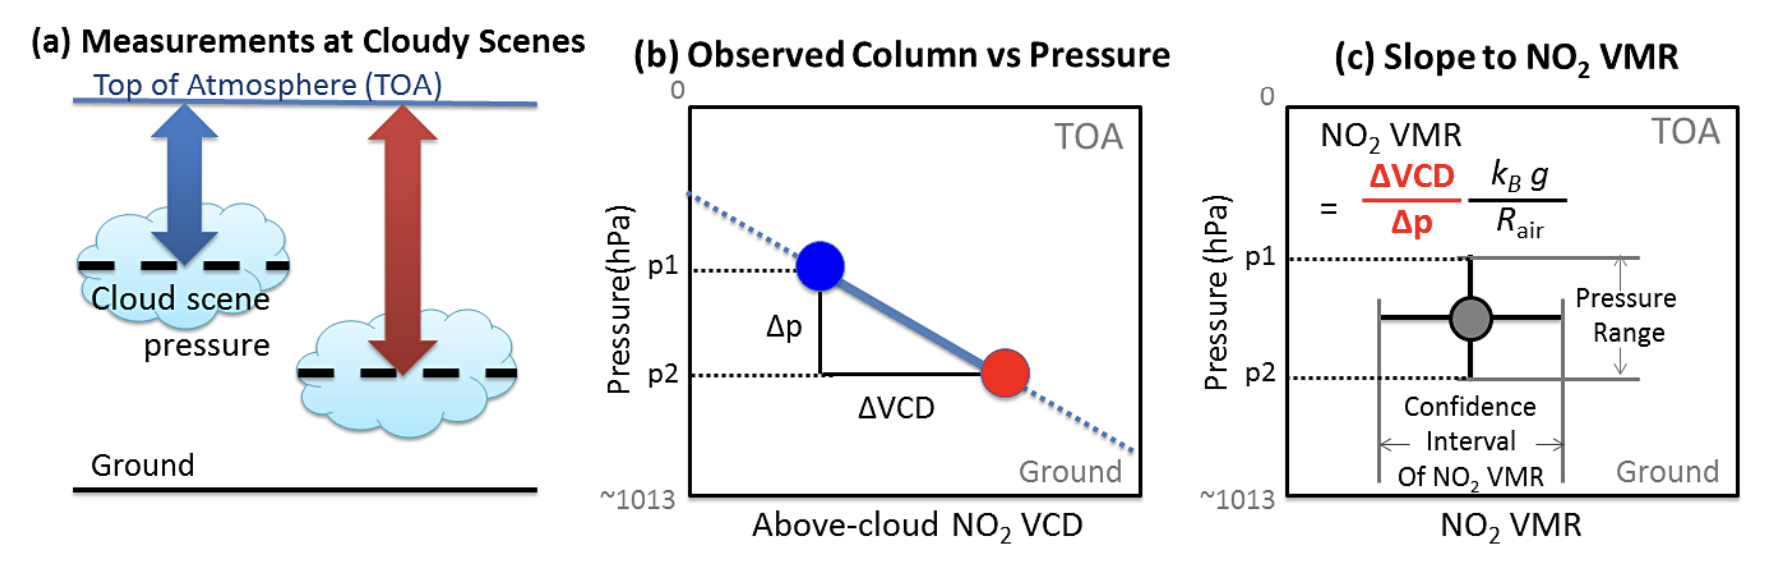
\includegraphics[width=\textwidth]{./figures/cloud-slicing_schematic.png}
\caption{云切片技术示意图(未按比例):(a)在不同云压条件下的两次云上NO$_{\ch{2}}$ 柱浓度测量(蓝色:云压低的柱浓度;红色:云压高的柱浓度);
(b)在气压柱坐标平面上显示的测量值; (c)NO$_{\ch{2}}$体积混合比(VMR)源自云上NO$_{\ch{2}}$垂直柱浓度(VCD)与云压的斜率,置信区间为水平误差条和气压范围为垂直误差条。[图片来源:\citet{Choi.2014}]\\
Figure \ref{fig:cloud-slicing_schematic}. Schematic view of the cloud-slicing technique (not to scale):
(a) two above-cloud NO$_{\ch{2}}$ column measurements at different cloud scene pressures (blue: column with lower scene pressure; and red: column with higher scene pressure);
(b) the measurements shown on a pressure-column coordinate plane;
(c) NO$_{\ch{2}}$ volume mixing ratios (VMR) derived from the slope of above-cloud NO$_{\ch{2}}$ vertical column densities (VCD) versus cloud scene pressure with confidence interval (horizontal error bar) and pressure range (vertical error bar). [Image source: \citet{Choi.2014}]
}
\label{fig:cloud-slicing_schematic}
\end{figure}

从这个关系式可以看出,TROPOMI云压范围内的$VMR_{\ch{NO2}}$与$V_{\ch{NO2Vis}}$和$p_{cloud}$的拟合斜率成正比(图\ref{fig:cloud-slicing_schematic}c)。
如果有两个以上的观测值,则可以从线性拟合中推导出$VMR_{\ch{NO2}}$的置信区间,
即图\ref{fig:cloud-slicing_schematic}c中$VMR_{\ch{NO2}}$的云压范围(垂直误差条)以及置信区间(水平误差条)。
在本文中,我们利用TROPOMI、TM5和MERRA2-GMI数据生成了各自在2019年6--8月对流层各高度区间内的平均$VMR_{\ch{NO2}}$,其中$p_{cloud}$位于以 330、450、570、670、770 和 870 hPa 为底的云压区间内。
由于TM5的NO$_{\ch{2}}$为TROPOMI NO$_{\ch{2}}$的附属产品,
故利用与下文TROPOMI相同的筛选条件进行数据筛选。
而MERRA2-GMI则选择当地时下午2点的模拟数据,计算每个云层区间内的最大云量,若某区间内的最大云量$>$ 0.4,则判断该区间为多云,并计算平均$VMR_{\ch{NO2}}$。

具体而言,$V_{\ch{NO2Vis}}$有两种计算方法:
1)基于近朗伯多云AMF假设,即具有较大总光学深度的散射云均匀分布在薄层上\citep{Choi.2014};
2)几何AMF,即$AMF_{\ch{geo}}$ = sec(SZA) + sec(VZA),其中 SZA 和 VZA 分别是太阳和视角天顶角\citep{Marais.2018,Marais.2021}。
由于对流层上层中NO$_{\ch{2}}$垂直分布的不确定性\citep{Travis.2016},我们使用$AMF_{\ch{geo}}$来计算云切片方法需要的$V_{\ch{NO2Vis}}$。
\citet{Choi.2014}的研究表明,该计算方法得到的$V_{\ch{NO2Vis}}$在对流层中层(650 hPa)最多比近朗伯多云AMF方法计算的结果高14\%。
因此,云切片算法中的$V_{\ch{NO2Vis}}$表达式如下:
\begin{equation} \label{eq:AMF_geo}
\begin{split}
V_{\ch{NO2Vis}} & = \frac{S_{\ch{NO2}}}{AMF_{\ch{geo}}} \\
             & = \frac{S_{\ch{total}}-(V_{\ch{strat}} \cdot AMF_{\ch{strat}})}{\sec (\mathrm{SZA})+\sec (\mathrm{VZA})}
\end{split}
\end{equation}
其中$S_{\ch{total}}$是总NO$_{\ch{2}}$斜柱浓度,$V_{\ch{strat}}$为平流层NO$_{\ch{2}}$垂直柱浓度,$AMF_{\ch{strat}}$为平流层空气质量分子。


虽然云切片方法无需知道具体的平流层NO$_{\ch{2}}$柱浓度即可推导出对流层的$VMR_{\ch{NO2}}$,但它依赖于以下假设和条件:
1)有相对大量的多云像素处于邻近位置,且这些像素具有足够的云压变化;
2)NO$_{\ch{2}}$在给定的云压和空间范围内,需在垂直和水平方向上充分混合;
3)平流层柱浓度在像素区域内保持不变;
4)计算得到的$VMR_{\ch{NO2}}$绝对量级仅与$V_{\ch{NO2Vis}}$具有一样的准确度,云压也可能会带来额外的不确定性。
因此,我们参考\citet{Marais.2021}设置了以下条件来获得有效的云切片结果。
首先将SZA $\geq$ 80$^{\circ}$ 和表面反照率 $\geq$  30\%的像素数据去除。
接着提取多云的像素[云辐射分数(CRF)$>$ 0.7],以最大限度地减少来自对流层下层的污染。
然后将每日的像素分配到1$^{\circ}$ $\times$ 1$^{\circ}$的网格中,保留满足云压具有足够大的变化范围[云压距离 $>$ 0.5*(最高云的气压 - 最低云的气压),且标准差$>$ 30 hPa]和充分混合的NO$_{\ch{2}}$(NO$_{\ch{2}}$ 垂直梯度 < 0.33 pptv hPa$^{-1}$)的像素。
若网格中像素个数超过10,则将得到的$VMR_{\ch{NO2}}$赋值到该日的网格点,最后可得到各高度的季节平均$VMR_{\ch{NO2}}$。

\section{痕量气体的垂直分布}

\subsection{二氧化氮}  \label{sec:no2_profile}


图\ref{fig:no2geo_tropomi}为TROPOMI观测的2019年中低纬度云上NO$_{\ch{2}}$柱浓度分布图,
气压区间分别为对流层顶--330 hPa、330--450 hPa、
450--570 hPa、570--670 hPa、670--770 hPa和770--870 hPa。
其中对流层顶--330 hPa和330--450 hPa的云上NO$_{\ch{2}}$高值区位于北美东北部、中国沿海地区、中国华北地区、墨西哥、
孟加拉国、尼泊尔、新德里、非洲中部和热带辐合带,
这些地区与图\ref{fig:no2_ltngcount}c中的闪电高值区相对应。
前人研究表明,中低纬LNO$_{\ch{2}}$的峰值分布在100--500 hPa之间\citep{Pickering.1988,Ott.2010,Luo.2017},
故对流层顶--450 hPa的云上NO$_{\ch{2}}$包含了LNO$_{\ch{2}}$的贡献。
然而TROPOMI的晴空NO$_{\ch{2}}$平均柱浓度产品显示这些地区属于NO$_{\ch{2}}$高污染区(图\ref{fig:no2_ltngcount}b),
所以云压处于对流层上层的NO$_{\ch{2}}$柱浓度也有来自深对流垂直输送的污染NO$_{\ch{2}}$。
中云(450--670 hPa)的云上NO$_{\ch{2}}$柱浓度有效数据更多,
其高值区包含了高云(对流层顶--450 hPa)的云上NO$_{\ch{2}}$柱浓度高值区。
其中污染NO$_{\ch{2}}$的贡献更为明显,与晴空NO$_{\ch{2}}$平均柱浓度产品分布更为接近,
如中国东部、欧洲和北美东北部的工业源以及非洲中部的生物质燃烧。
污染物排放在低云(670--870 hPa)的云上NO$_{\ch{2}}$柱浓度分布中最为明显,然而由于热带地区云顶较高,有效数据更少。



\begin{figure}[H]
    \centering
    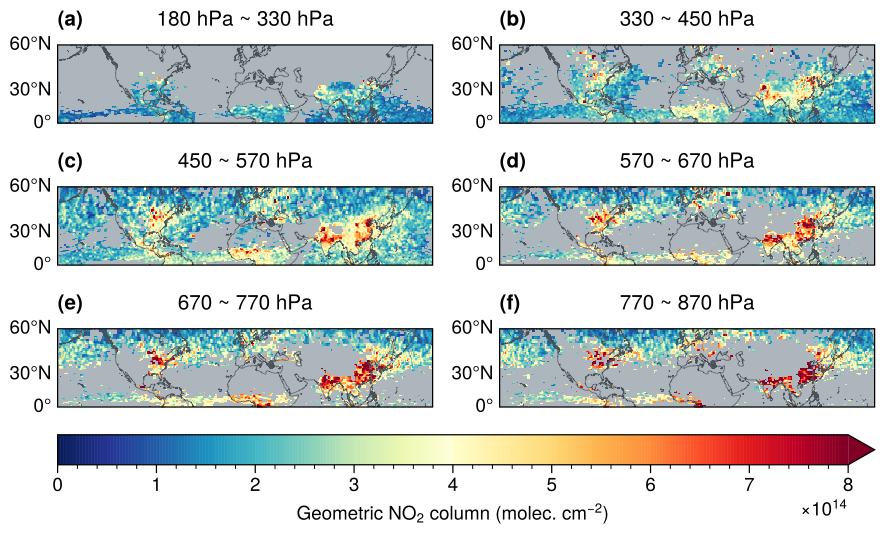
\includegraphics[width=0.9\textwidth]{./figures/no2geo_tropomi.png}
    \caption{
    2019年6--8月北半球中低纬度TROPOMI观测的云上NO$_{\ch{2}}$柱浓度分布图:
    高云[(a)对流层顶 --330 hPa 和(b)330--450 hPa],
    中云 [(c)450--570 hPa 和(d)570--670 hPa],
    及低云 [(e) 670--770 hPa 和(f)770--870 hPa]。 \\
    Figure \ref{fig:no2geo_tropomi}. NO$_{\ch{2}}$ above cloud at the middle-low latitudes for June--August in 2019:
    High clouds [(a) tropopause--330 hPa, (b) 330--450 hPa],
    middle clouds [(c) 450--570 hPa, (d) 570--670 hPa],
    and low clouds [(e) 670--770 hPa, (f) 770--870 hPa].
    }
    \label{fig:no2geo_tropomi}
\end{figure}

\begin{figure}[H]
    \centering
    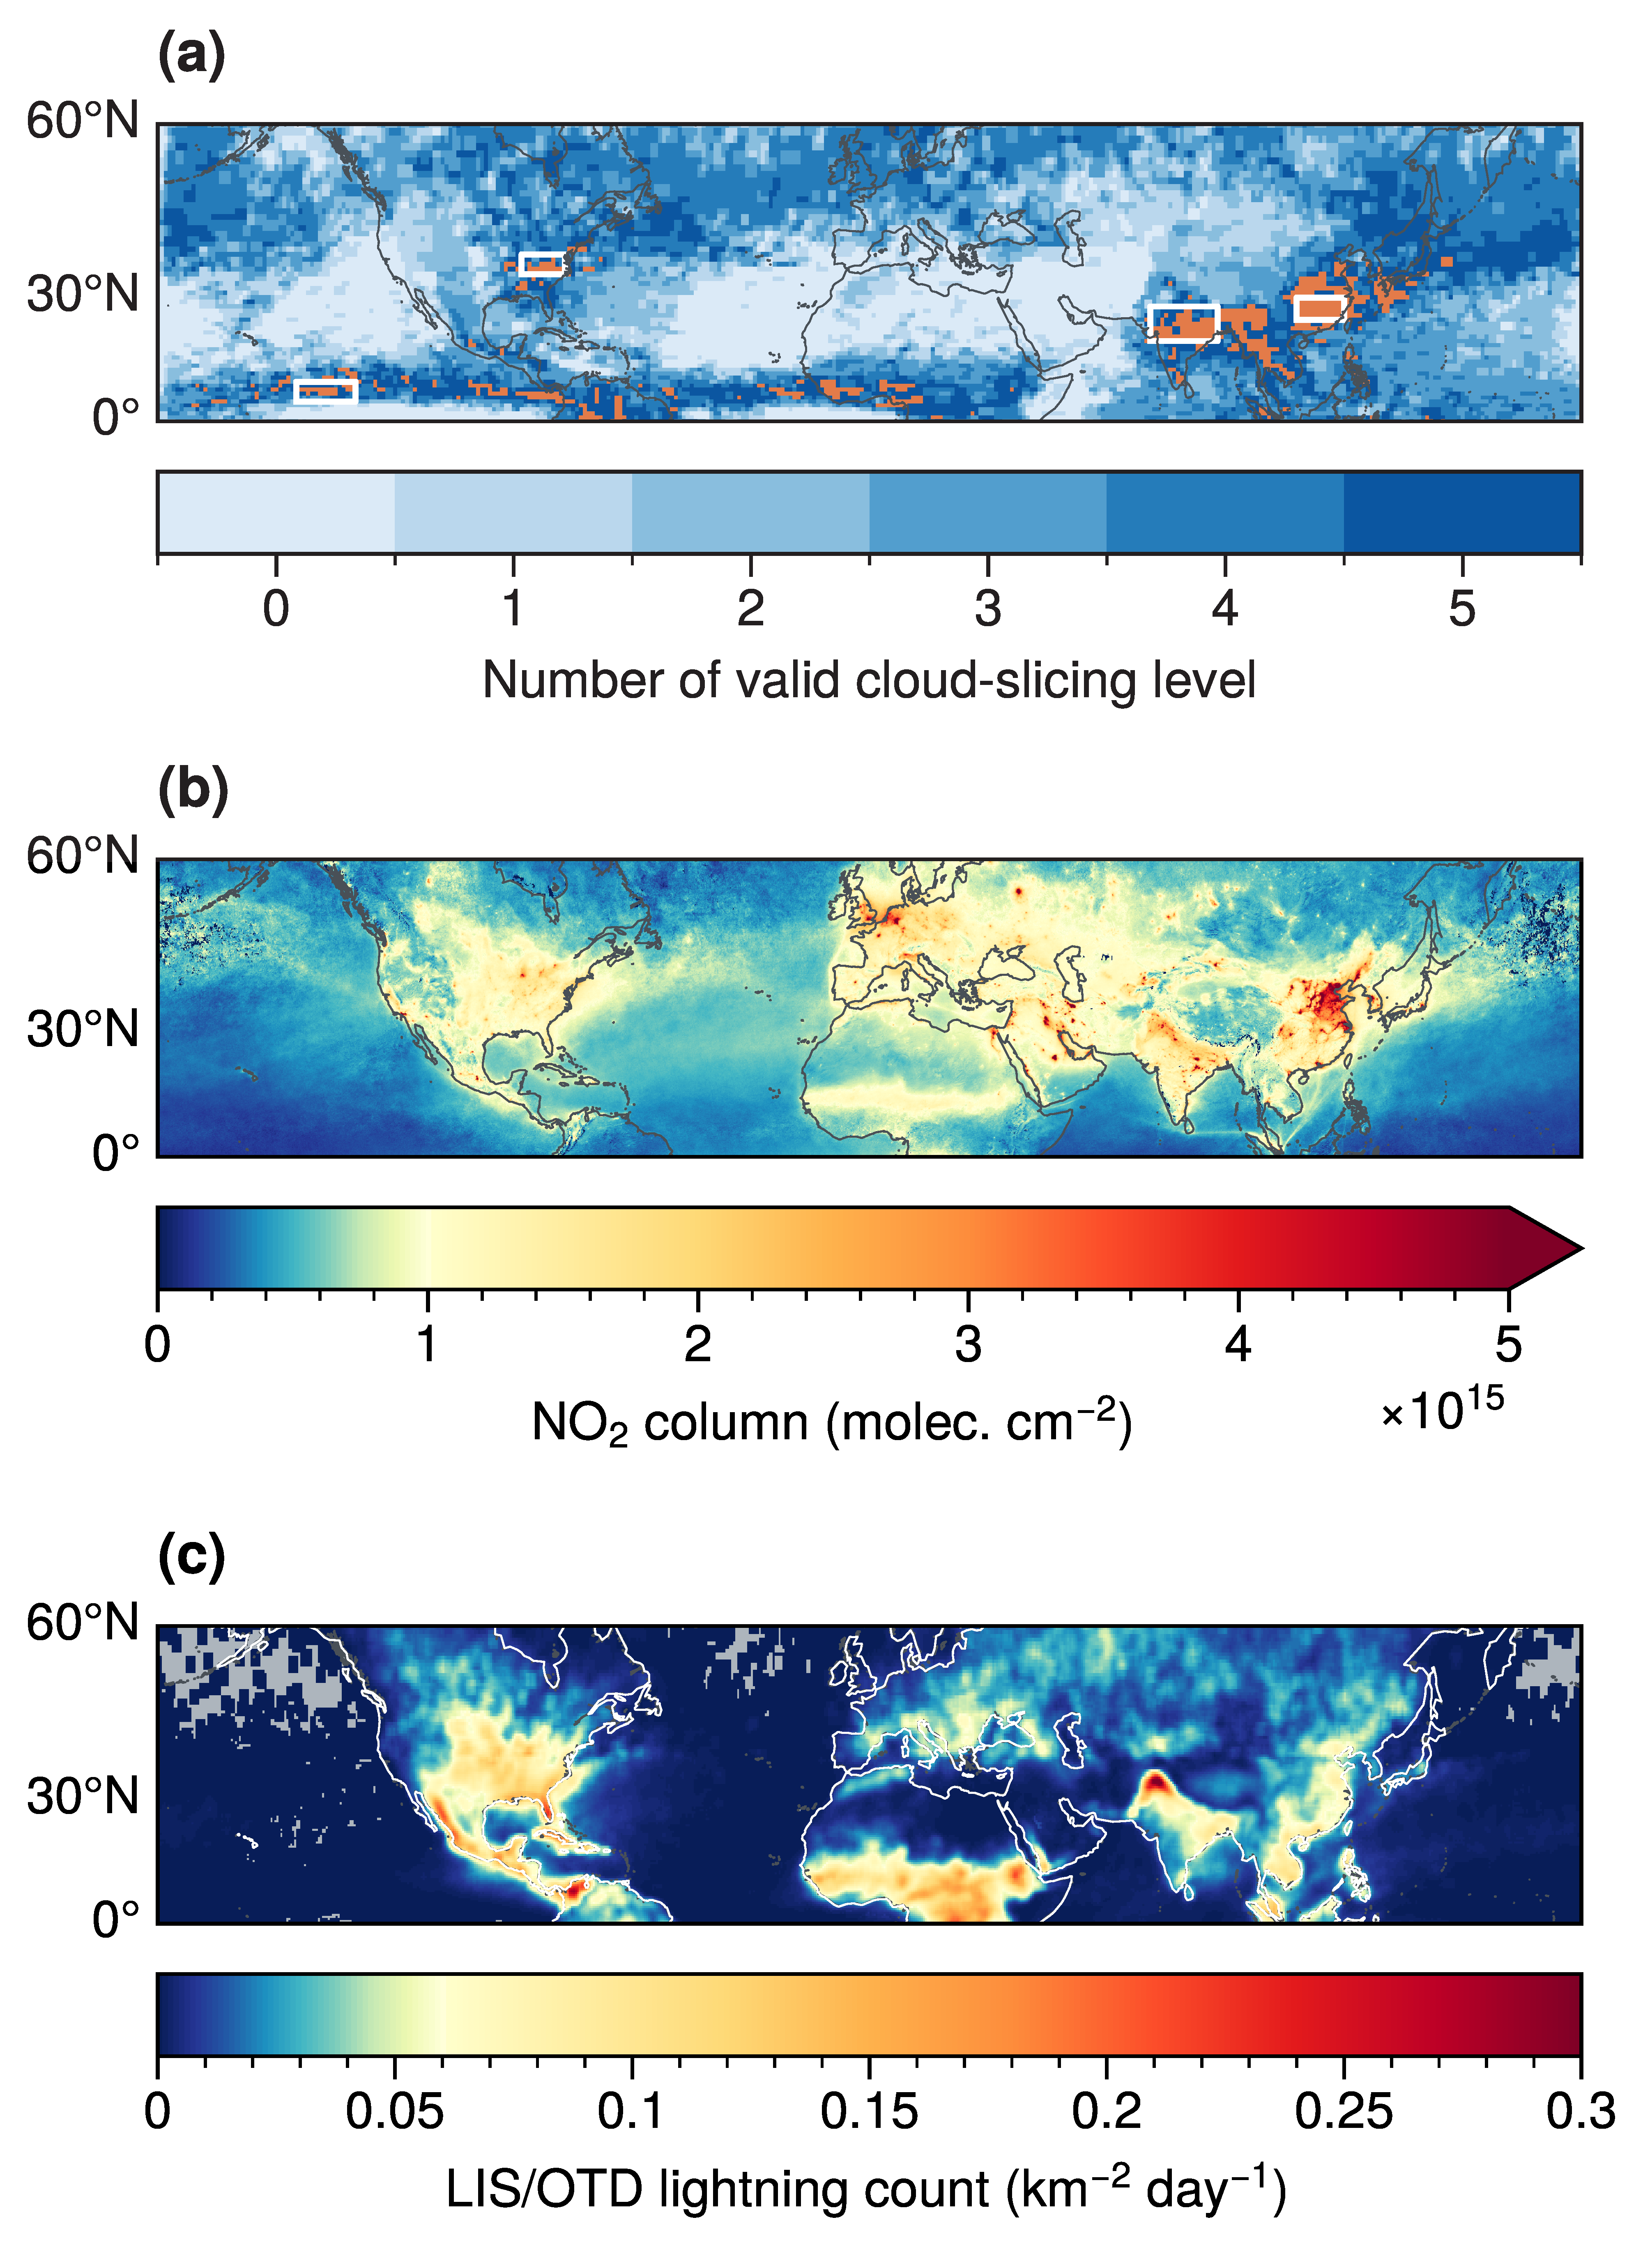
\includegraphics[width=0.7\textwidth]{./figures/no2_ltngcount.png}
    \caption{
    (a)云切片的总有效气压层数,层数$\leq$ 5为蓝色,= 6 为橙色,白色方框为NO$_{\ch{2}}$廓线选区(图\ref{fig:utno2_profile});
    (b)2019--2021年中低纬度夏季(6--8月)TROPOMI测得的NO$_{\ch{2}}$平均柱浓度;
    (c)1995--2014年中低纬度夏季(6--8月)LIS/OTD的闪电密度产品。 \\
    Figure \ref{fig:no2_ltngcount}. (a) Number of total valid cloud-slicing pressure levels.
    Grids with number of levels $\leq$ 5 and = 6 are filled in blue and orange, respectively.
    White rectangles are selections for NO$_{\ch{2}}$ profiles (Fig. \ref{fig:utno2_profile}).
    (b) The average TROPOMI NO$_{\ch{2}}$ column densities at the middle-low latitudes for June--August in 2019--2021.
    (c) The average LIS/OTD lightning flash rates at the middle-low latitudes for June--August in 1995--2014.
    }
    \label{fig:no2_ltngcount}
\end{figure}


利用\ref{sec:cloud-slicing}节的云切片算法,可进一步得到每层的NO$_{\ch{2}}$浓度,即NO$_{\ch{2}}$廓线。
图\ref{fig:utno2_tropomi}为2019年6--8月不同高度的NO$_{\ch{2}}$平均浓度。
与图\ref{fig:no2geo_tropomi}的云上NO$_{\ch{2}}$柱浓度不同,
高云处的NO$_{\ch{2}}$浓度(图\ref{fig:utno2_tropomi}a,b)高于中云(图\ref{fig:utno2_tropomi}c,d)。
其中陆地上对流层顶--330 hPa间的NO$_{\ch{2}}$浓度为330--450 hPa间的$\sim$1.2倍,为450--570 hPa间的$\sim$2倍,
而570 hPa以下(图\ref{fig:utno2_tropomi}d--f)陆地上的NO$_{\ch{2}}$浓度逐渐上升。
该现象与前人的模式模拟和飞机观测结果相符:LNO$_{\ch{2}}$在对流层上层占主导,
而人为污染NO$_{\ch{2}}$在对流层下层占主导\citep{Pickering.1996,Ott.2010,Laughner.2017}。


\begin{figure}[H]
    \centering
    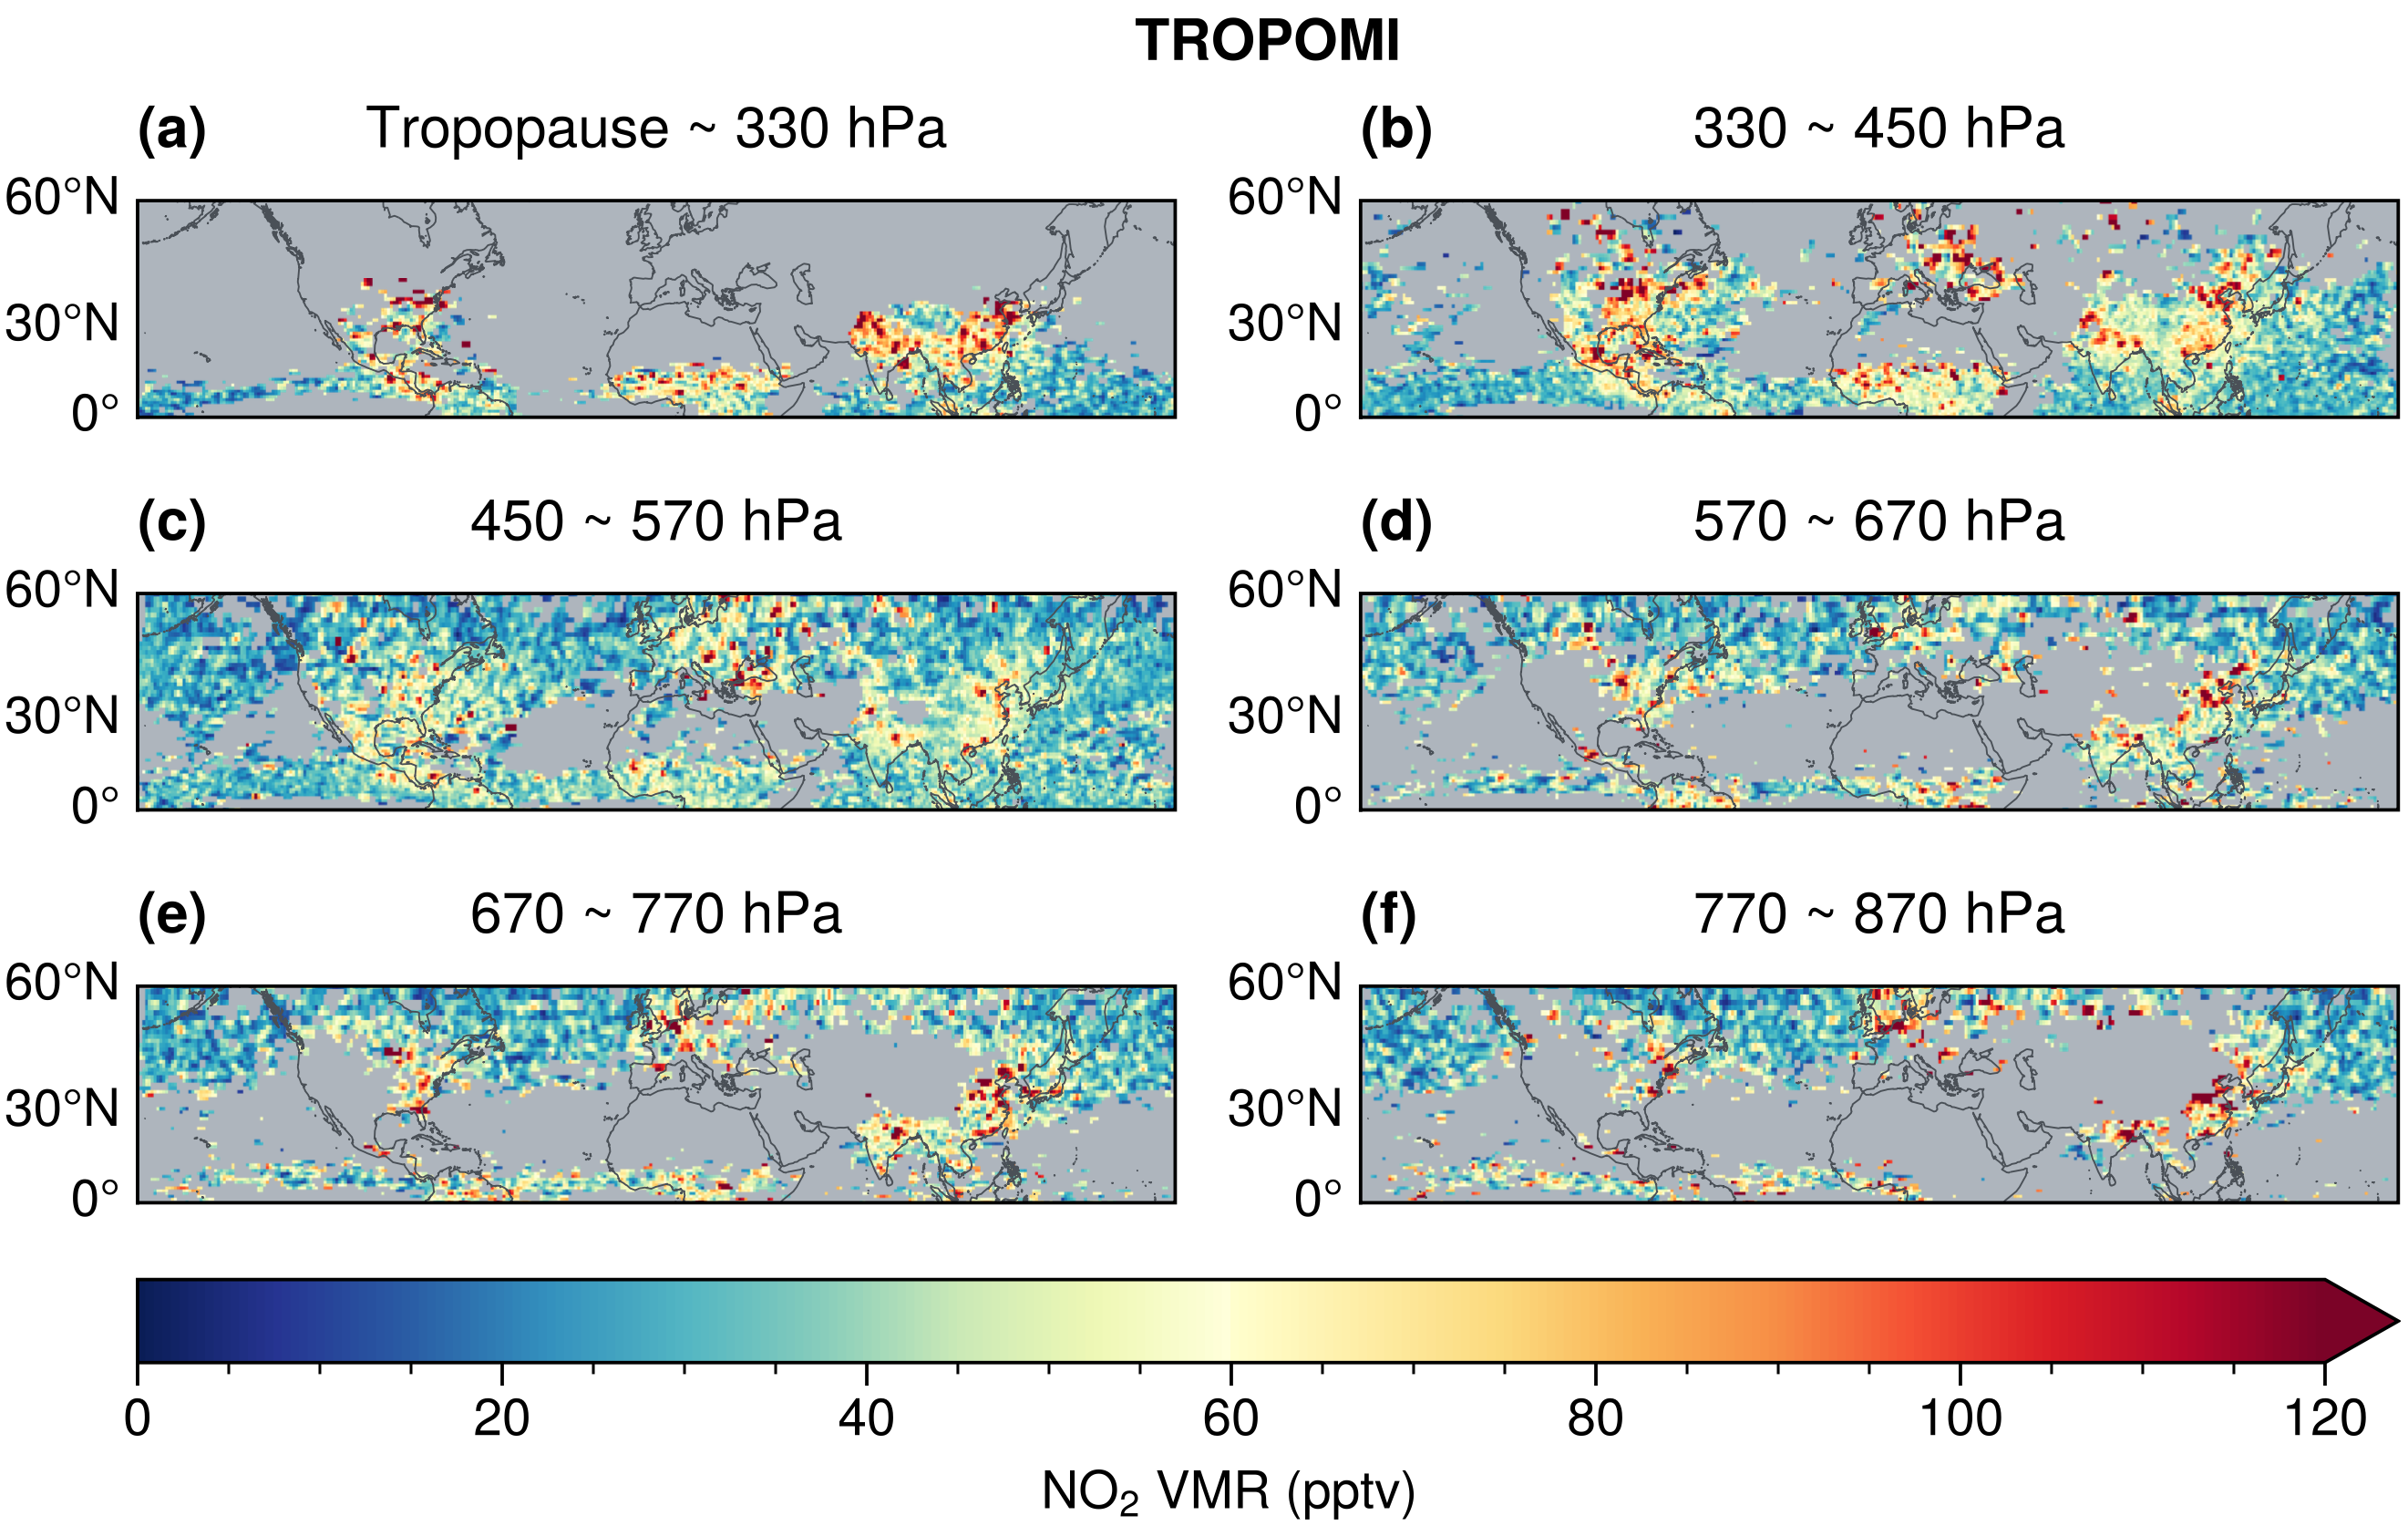
\includegraphics[width=0.9\textwidth]{./figures/utno2_tropomi.png}
    \caption{
    TROPOMI云切片算法所得的2019年6--8月北半球中低纬度NO$_{\ch{2}}$浓度分布图。 \\
    Figure \ref{fig:utno2_tropomi}. The NO$_{\ch{2}}$ vertical mixing ratios derived from the cloud-slicing results of TROPOMI NO$_{\ch{2}}$ observations at the northern middle-low latitudes for June--August in 2019.
    }
    \label{fig:utno2_tropomi}
\end{figure}

为了进一步分析LNO$_{\ch{2}}$在其中的作用,我们首先将各个高度层的TROPOMI观测结果与MERRA2-GMI的模式结果相比较,
接着选取TROPOMI云切片各层均有有效数据的区域,结合过境期间模拟的LNO$_{\ch{2}}$排放速率垂直分布进行廓线分析。
图\ref{fig:utno2_merra2}为2019年6--8月与TROPOMI对应的MERRA2-GMI NO$_{\ch{2}}$模拟结果,
% 由两者浓度之差(TROPOMI - MERRA2-GMI,图\ref{fig:utno2_delta})可知,无论位于陆地还是海洋,MERRA2-GMI较TROPOMI存在20--80 pptv的低估,
图\ref{fig:utno2_delta}为两者浓度之差(TROPOMI - MERRA2-GMI)的分布图。
其中海洋上的误差可能由TROPOMI NO$_{\ch{2}}$反演过程中低估的平流层NO$_{\ch{2}}$柱浓度或高估的辐射强度所导致\citep{VanGeffen.2020}。

具体而言,高云间的NO$_{\ch{2}}$正误差为28 $\pm$ 19 pptv,
% 即高云间MERRA2-GMI模拟的NO$_{\ch{2}}$比TROPOMI的观测值低25\%,
主要位于北美、东欧以及亚洲东部沿海(图\ref{fig:utno2_delta}a,b),
这意味着MERRA2-GMI全球模式中参数化对流垂直传输污染物的强度可能偏低。
而高云间的NO$_{\ch{2}}$负误差(-12 $\pm$ 11 pptv)位于美国中部、非洲中部以及青藏高原西南部。
美国中部和非洲中部的误差是由于MERRA2-GMI中的闪电参数化(对流层上层的向上云质量通量)高估了该区域的闪电总量,从而导致NO$_{\ch{2}}$浓度偏大\citep{Allen.2002,Allen.2010}。
由LIS/OTD闪电观测数据(图\ref{fig:no2_ltngcount}c)可知,
青藏高原西南部闪电强度较弱,故模式的高估主要应来自于亚洲夏季风的污染物输送。

中云的云切片结果有效范围最广,总体上来看TROPOMI和MERRA2-GMI之间误差较低(18 $\pm$ 17 pptv),
且两者具有相似的高值区分布:北美、东欧、印度以及中国华北地区,这些地区与污染NO$_{\ch{2}}$柱浓度高值区对应。
中云高度的NO$_{\ch{2}}$可能来源有对流输送的地表污染和污染的出流区,如中国华北地区的NO$_{\ch{2}}$高值传输至东部的黄海(其中一部分也来自于船舶排放)。
其中$>$ 40 pptv的正误差集中于南美洲北部、缅甸和泰国北部,由于这些地区地基NO$_{\ch{2}}$观测资料稀缺,
所以该误差应归因于卫星反演误差还是模式NO$_{\ch{x}}$排放源的不确定性,还有待进一步研究。
此外,中云的负误差结果在570--670 hPa更为明显(-10 $\pm$ 15 pptv),尤其是中国的华北地区,
考虑到MERRA2-GMI对流垂直输送强度较低,故使用的排放清单中NO$_{\ch{x}}$排放量可能过高\citep{Ziemke.2019}。

\begin{figure}[H]
    \centering
    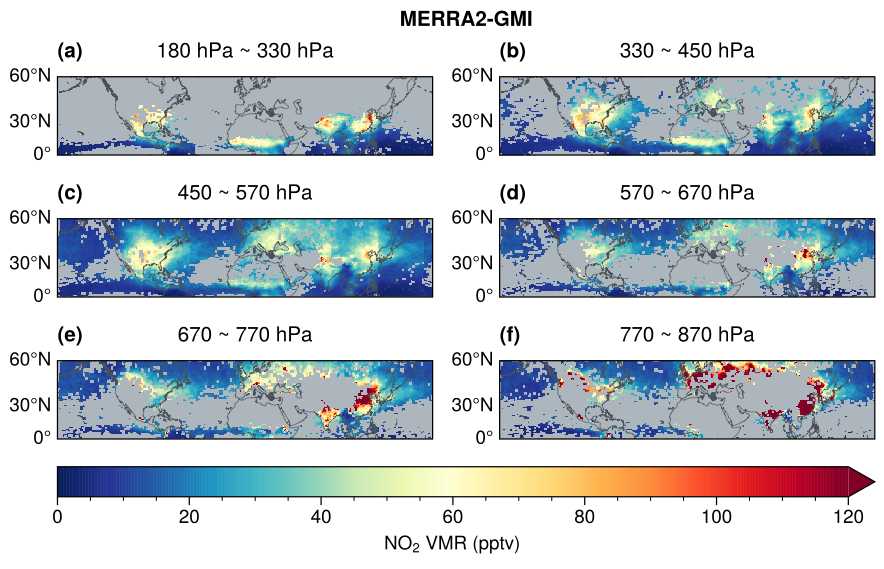
\includegraphics[width=0.9\textwidth]{./figures/utno2_merra2-gmi.png}
    \caption{
    同图\ref{fig:utno2_tropomi}但数据为MERRA2-GMI。 \\
    Figure \ref{fig:utno2_merra2}. Same as Fig. \ref{fig:utno2_tropomi} but for MERRA2-GMI.
    }
    \label{fig:utno2_merra2}
\end{figure}

低云的云切片NO$_{\ch{2}}$高值区与中云结果类似,
总体上来看TROPOMI和MERRA2-GMI之间误差较大(15 $\pm$ 50 pptv),
在中国东部和印度北部的负误差最为明显($<$-100 pptv)。
前人研究表明,本研究中所用的几何AMF(AMF$_{geo}$,式\ref{eq:AMF_geo})在低云和污染条件下可达可见AMF(AMF$_{Vis}$,式\ref{eq:AMF_NO2Vis})的两倍\citep{BelmonteRivas.2015},然而这不足以解释中国东部地区的模拟值为观测值的3--5倍。
因此,该差异反映了MERRA2-GMI使用的MACCity排放清单在中国东部未能及时更新。


\begin{figure}[H]
    \centering
    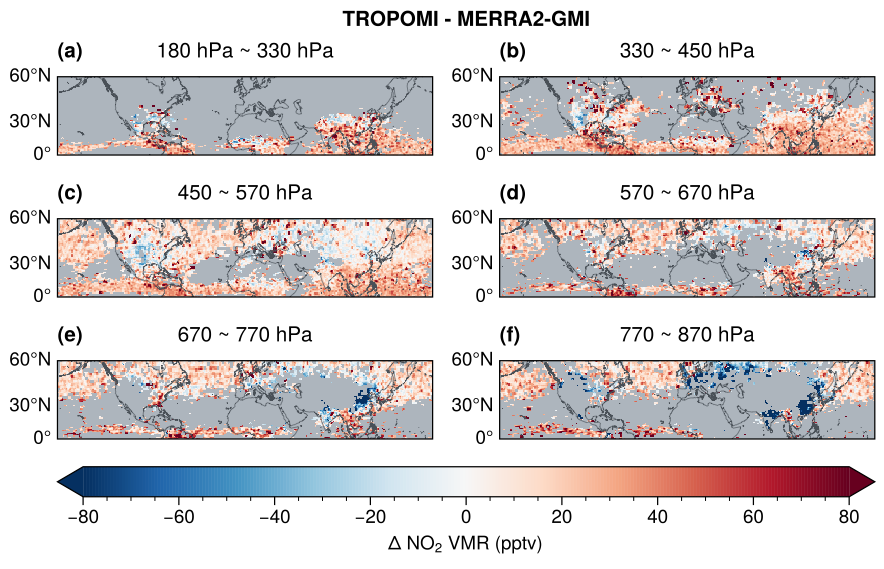
\includegraphics[width=0.9\textwidth]{./figures/utno2_delta.png}
    \caption{
    图\ref{fig:utno2_tropomi}与图\ref{fig:utno2_merra2}之差。 \\
    Figure \ref{fig:utno2_delta}. Differences between Fig. \ref{fig:utno2_tropomi} and Fig. \ref{fig:utno2_merra2}.
    }
    \label{fig:utno2_delta}
\end{figure}



除了各层NO$_{\ch{2}}$浓度的地理分布之外,我们选取了区域内云切片有效层数为6层的格点
(分别位于中国南部、印度中部、美国东南部以及太平洋,图\ref{fig:no2_ltngcount}a),
进行TM5、MERRA2-GMI和TROPOMI的廓线对比分析,
其中TM5的NO$_{\ch{2}}$廓线为TROPOMI官方产品使用的TM5全球模式先验廓线(包含TROPOMI同化)。
由于TROPOMI在太平洋清洁地区的高估,我们将云切片结果进行校正,即除以其与MERRA2-GMI和TROPOMI比例的平均值。
如图\ref{fig:utno2_profile}所示,太平洋清洁地区NO$_{\ch{2}}$在对流层各层浓度分布均一(2.5--12.5 pptv),
中国南部和印度中部低层NO$_{\ch{2}}$污染浓度高(200--300 pptv),而美国东南部低层NO$_{\ch{2}}$浓度为50--100 pptv。
由于污染地区对流层低层TROPOMI NO$_{\ch{2}}$浓度存在与图\ref{fig:utno2_delta}中类似的低估,故只比较三者在对流层中上层的NO$_{\ch{2}}$浓度大小。


\begin{figure}[H]
    \centering
    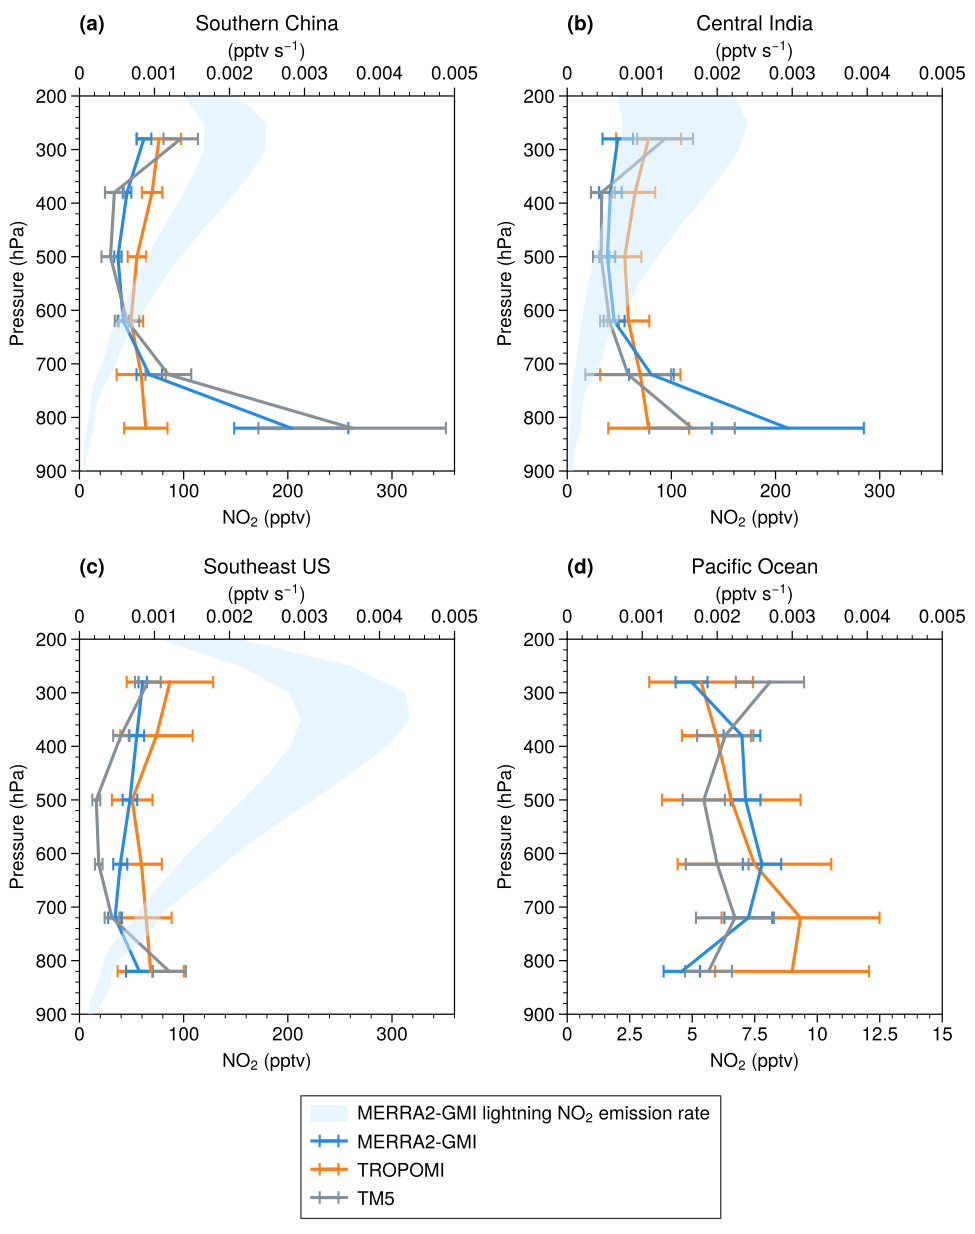
\includegraphics[width=0.9\textwidth]{./figures/utno2_profile.png}
    \caption{
    TM5(灰色)、MERRA2-GMI(蓝色)以及TROPOMI云切片算法(橙色)所得到的区域平均NO$_{\ch{2}}$廓线:
    (a)中国南部、(b)印度中部、(c)美国东南部、(d)太平洋(区域示意图见图\ref{fig:no2_ltngcount}a)。
    浅蓝色填充部分为下午地方时2点的MERRA2-GMI闪电NO$_{\ch{2}}$排放速率,
    其中廓线的误差棒和填充范围为平均值$\pm$标准差。\\
    Figure \ref{fig:utno2_profile}. Regional average NO$_{\ch{2}}$ profiles obtained by TM5 (gray), MERRA2-GMI (blue), and TROPOMI cloud slice algorithm (orange).
    (a) southern China, (b) central India, (c) southeastern United States, and (d) Pacific Ocean
    (Definitions of region are shown in Fig. \ref{fig:no2_ltngcount}a).
    The light blue filled part is the MERRA2-GMI lightning NO$_{\ch{2}}$ emission rate at local 2 p.m.,
    where the error bars and filled ranges of the profiles are the mean values $\pm$ standard deviations.
    }
    \label{fig:utno2_profile}
\end{figure}


对于中国南部、印度中部和美国东南部,NO$_{\ch{2}}$廓线呈“C”形:NO$_{\ch{2}}$首先随高度而下降,
在500--600 hPa存在转折点,进而浓度上升,在对流层顶--300 hPa达到峰值($\sim$80 pptv)。
总体来看,对流层中上层MERRA2-GMI和TM5的NO$_{\ch{2}}$浓度相近,但均比TROPOMI的结果低,
表明模式中LNO$_{\ch{2}}$或对流输送的污染NO$_{\ch{2}}$存在低估,与前人的飞机探测和模式结果相符\citep{Laughner.2019a}。
具体而言,由于TM5的同化仅包含云上的信息,TM5的中上层拐点梯度更大,
其在对流层顶--330 hPa和330--450 hPa区间的NO$_{\ch{2}}$浓度比TROPOMI的观测结果分别低10\%和50\%,
而MERRA2-GMI结果较TROPMI的结果低30\%。
此外,MERRA2-GMI在美国东南部的LNO$_{\ch{2}}$排放速率为中国南部或印度中部的两倍,最上层的峰值浓度与TM5一致,
不同之处是浓度拐点降为700 hPa,该高度低于TM5和TROPOMI的500 hPa,
可能原因是MERRA2-GMI的美国东南部LNO$_{\ch{2}}$排放廓线在对流层中低层权重过高。
总之,TROPOMI的观测结果和MERRA2-GMI/TM5的模拟结果在对流层中上层存在显著的一致性,
局部的差异表明云切片方法可以用来检验模式的对流垂直输送和水平输送能力、使用的排放源清单以及LNO$_{\ch{x}}$的产量和分布。


\subsection{臭氧} \label{sec:o3_profile}

如图\ref{fig:uto3_tropomi}所示,云切片方法可得到2019年6--8月中低纬度对流云不同高度O$_{\ch{3}}$的平均浓度,
其有效范围比NO$_{\ch{2}}$的云切片结果(图\ref{fig:utno2_tropomi})更广,
尤其是在中云和高云条件下的中纬度地区(图\ref{fig:uto3_tropomi}b--d)。
这是由于TROPOMI的O$_{\ch{3}}$二级产品中云分数为光学云识别算法(OCRA)云分数,而NO$_{\ch{2}}$二级产品中使用从氧气A波段版本S(FRESCO-S)中快速检索云的方案。

总体来看,高云处的O$_{\ch{3}}$浓度(图\ref{fig:uto3_tropomi}a--b)高于中云(图\ref{fig:uto3_tropomi}c--d),
其中对流层顶--330 hPa间的O$_{\ch{3}}$为330--450 hPa间的$\sim$1.5倍,为450--570 hPa间的$\sim$2倍。
对于热带地区,非洲中部(20$^{\circ}$ W--50$^{\circ}$ E,0--20$^{\circ}$ N)的O$_{\ch{3}}$浓度比同纬度地区的O$_{\ch{3}}$浓度高,尤其是在中云和高云条件下可高出40--48\%,该现象与\citet{Cooper.2013}研究中215 hPa高度MLS的O$_{\ch{3}}$观测结果相符。
他们的研究指出,低O$_{\ch{3}}$事件经常发生在热带西太平洋,很少发生在热带其他地区,
而热带海洋区域在低O$_{\ch{3}}$事件和高云的频率之间存在一致的空间特征,表明这些事件来自于对流。
虽然非洲中部也是强对流频发地区,但生物质燃烧导致陆地边界层O$_{\ch{3}}$浓度往往高于海洋\citep{Thompson.2001,Anderson.2016},因此深对流产生较少的低O$_{\ch{3}}$事件。

\begin{figure}[H]
    \centering
    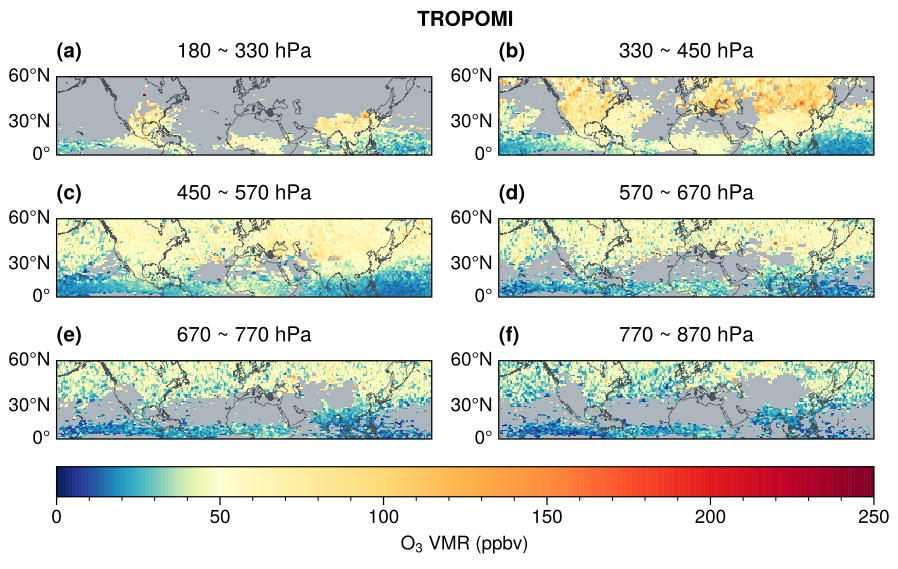
\includegraphics[width=0.95\textwidth]{./figures/uto3_tropomi.png}
    \caption{
    TROPOMI云切片算法所得的2019年6--8月北半球中低纬度O$_{\ch{3}}$浓度分布图。 \\
    Figure \ref{fig:uto3_tropomi}. The O$_{\ch{3}}$ vertical mixing ratios derived from the cloud-slicing results of TROPOMI O$_{\ch{3}}$ observations at the northern middle-low latitudes for June--August in 2019.
    }
    \label{fig:uto3_tropomi}
\end{figure}

为了进一步利用MERRA2-GMI的模式结果分析动力输送和化学反应在其中的作用,我们首先将各个高度的MERRA2-GMI模式结果与TROPOMI观测数据相比较。
图\ref{fig:uto3_merra2}为2019年6--8月与TROPOMI对应的MERRA2-GMI O$_{\ch{3}}$模拟结果,
图\ref{fig:uto3_delta}为TROPOMI与MERRA2-GMI在各层的结果之差($\Delta$ O$_{\ch{3}}$)。
总体上,非洲中部的$\Delta$ O$_{\ch{3}}$在中云和高云条件下为负(-23 $\pm$ 11 pptv,图\ref{fig:uto3_delta}a--d),
中纬度陆地地区的$\Delta$ O$_{\ch{3}}$在高云条件下为正(20 $\pm$ 15 pptv,图\ref{fig:uto3_delta}b)。
此外,$\Delta$ NO$_{\ch{2}}$(图\ref{fig:utno2_tropomi})和$\Delta$ O$_{\ch{3}}$(图\ref{fig:uto3_delta})的对比显示,
尽管中云和高云条件下NO$_{\ch{2}}$在大部分陆地地区被高估,但是O$_{\ch{3}}$却被低估。
\citet{Pickering.1990}于美国中南部清洁地区的研究显示,11 km处的LNO峰值排放导致该高度层为VOC控制区。
由于本研究全球模式中除化学反应外,动力输送也存在偏差,故不能确定是否为VOC控制区,有待将来进一步的研究。
低云条件下云切片算法低估O$_{\ch{3}}$的现象,也反映了AMF$_{\ch{geo}}$在低云和污染条件下的高估\citep{BelmonteRivas.2015}。


\begin{figure}[H]
    \centering
    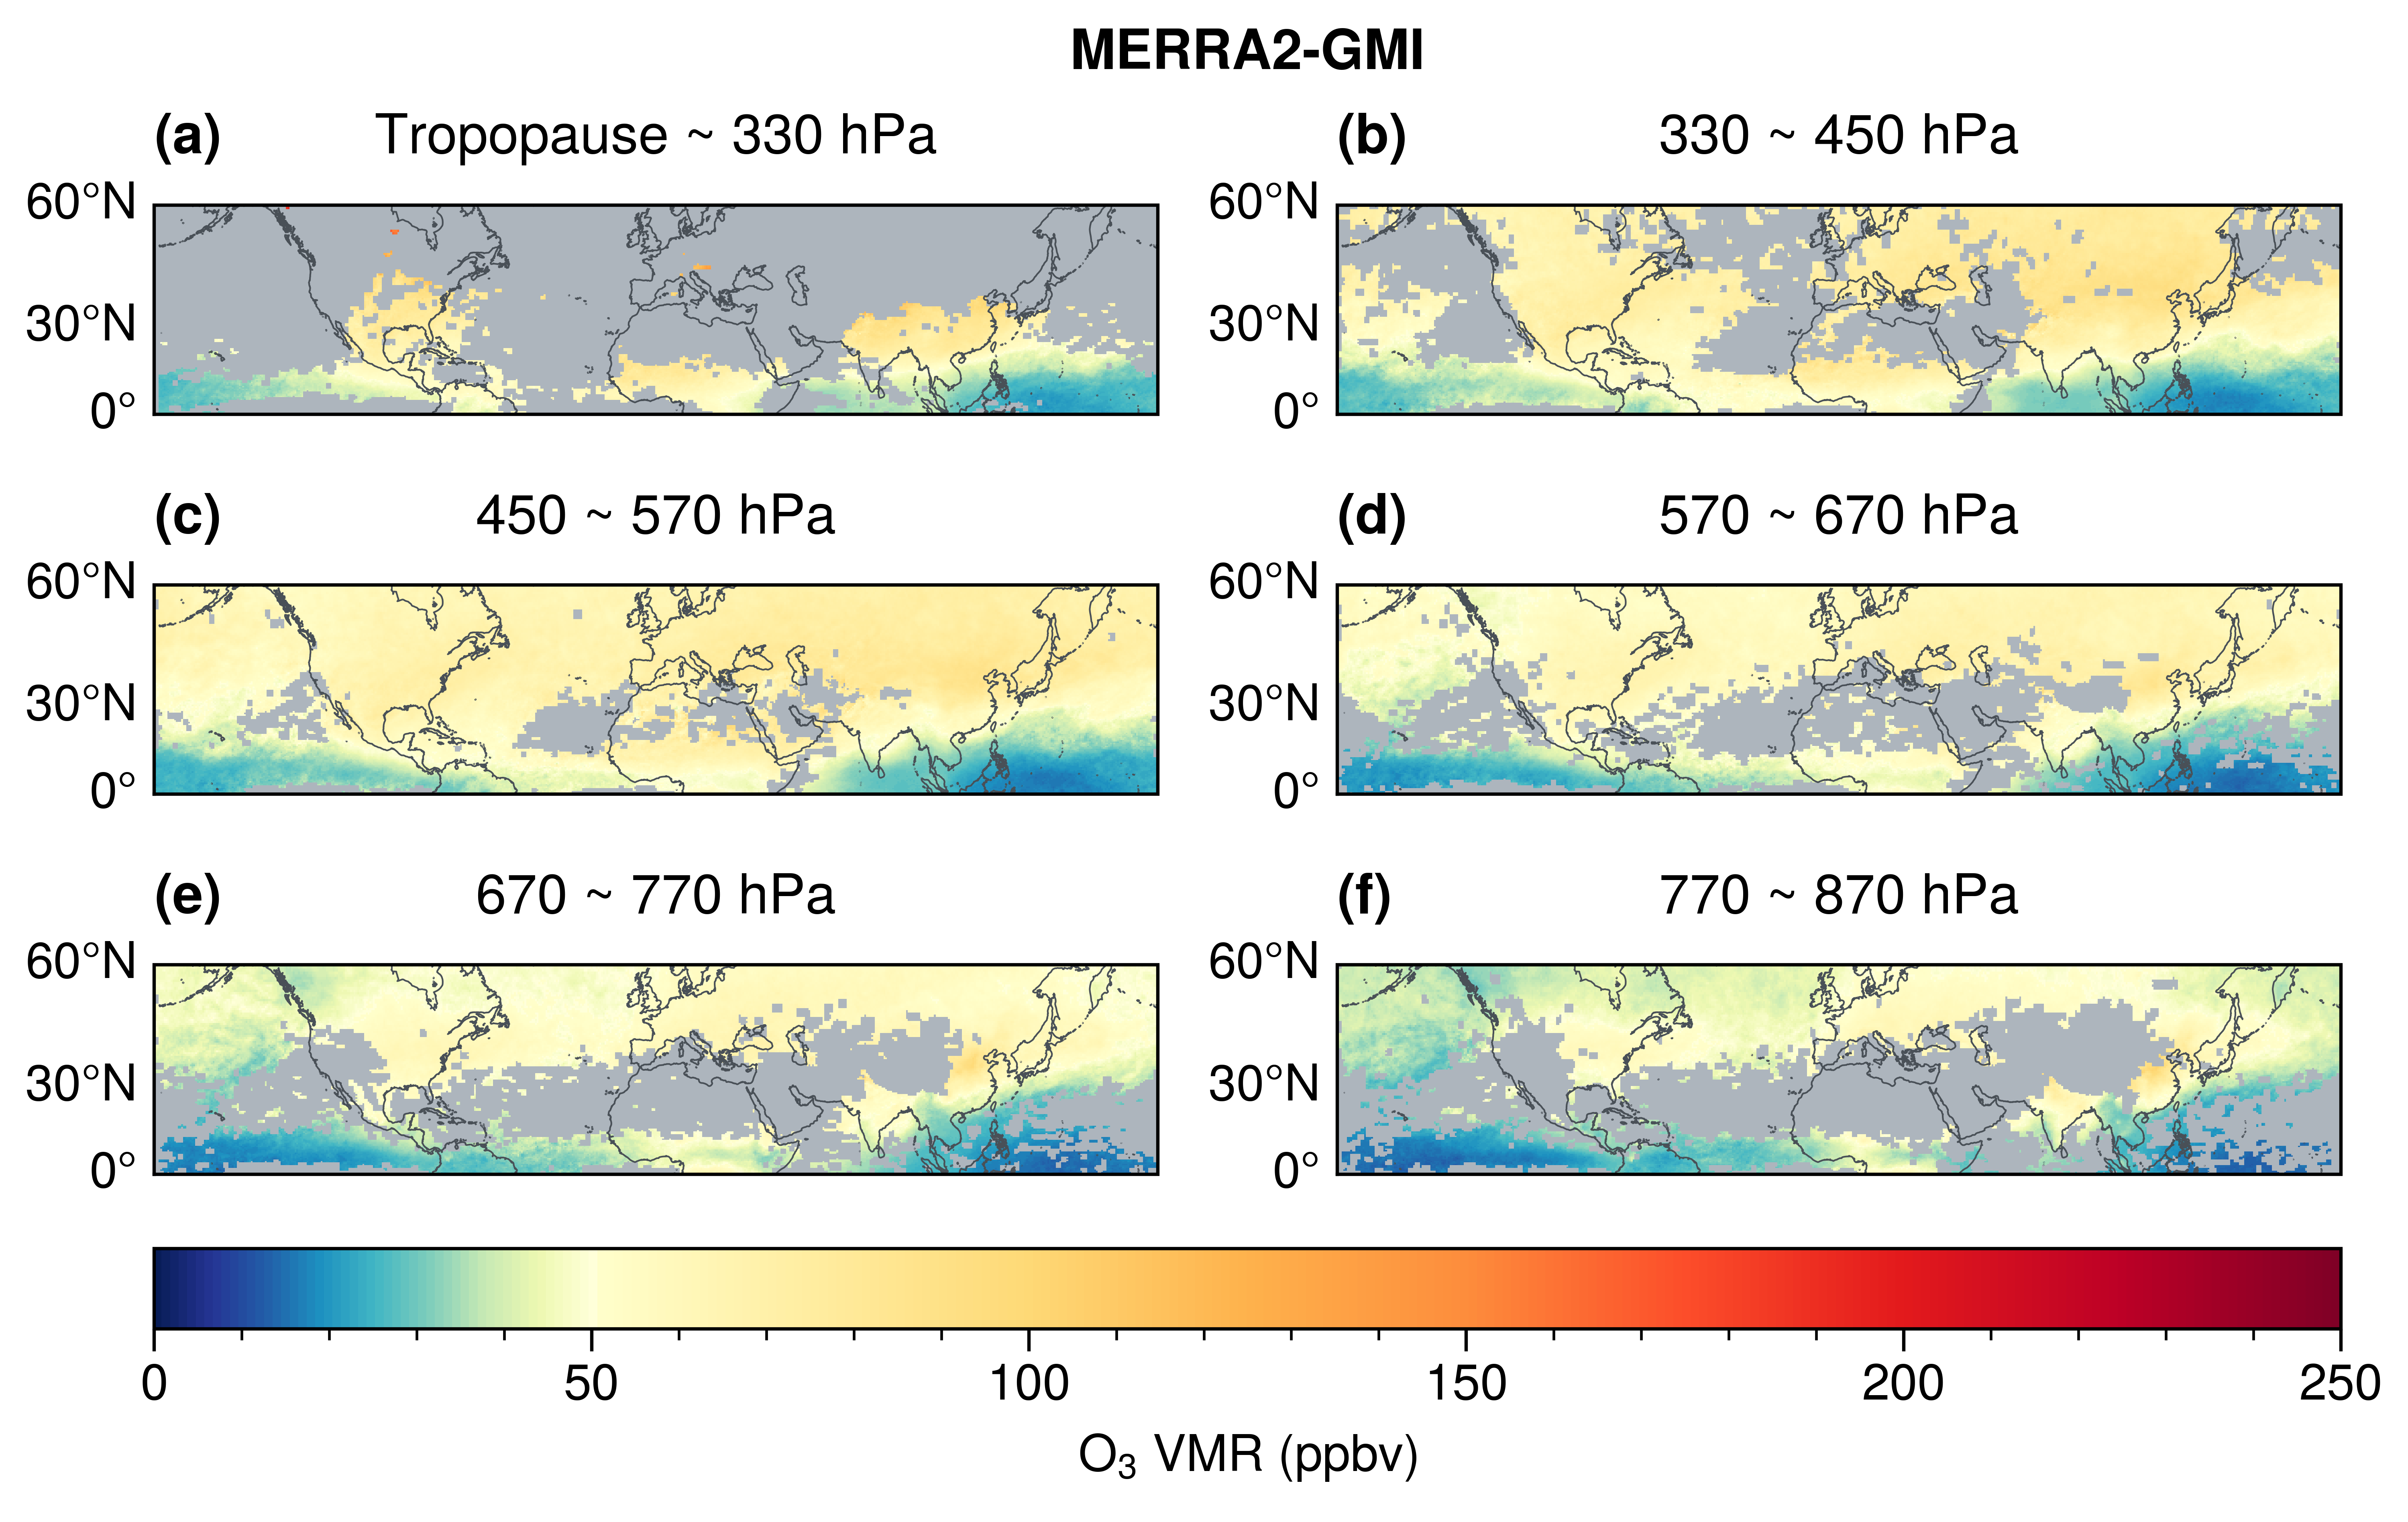
\includegraphics[width=0.9\textwidth]{./figures/uto3_merra2-gmi.png}
    \caption{
    同图\ref{fig:uto3_tropomi}但数据为MERRA2-GMI。 \\
    Figure \ref{fig:uto3_merra2}. Same as Fig. \ref{fig:uto3_tropomi} but for MERRA2-GMI.
    }
    \label{fig:uto3_merra2}
\end{figure}


\begin{figure}[H]
    \centering
    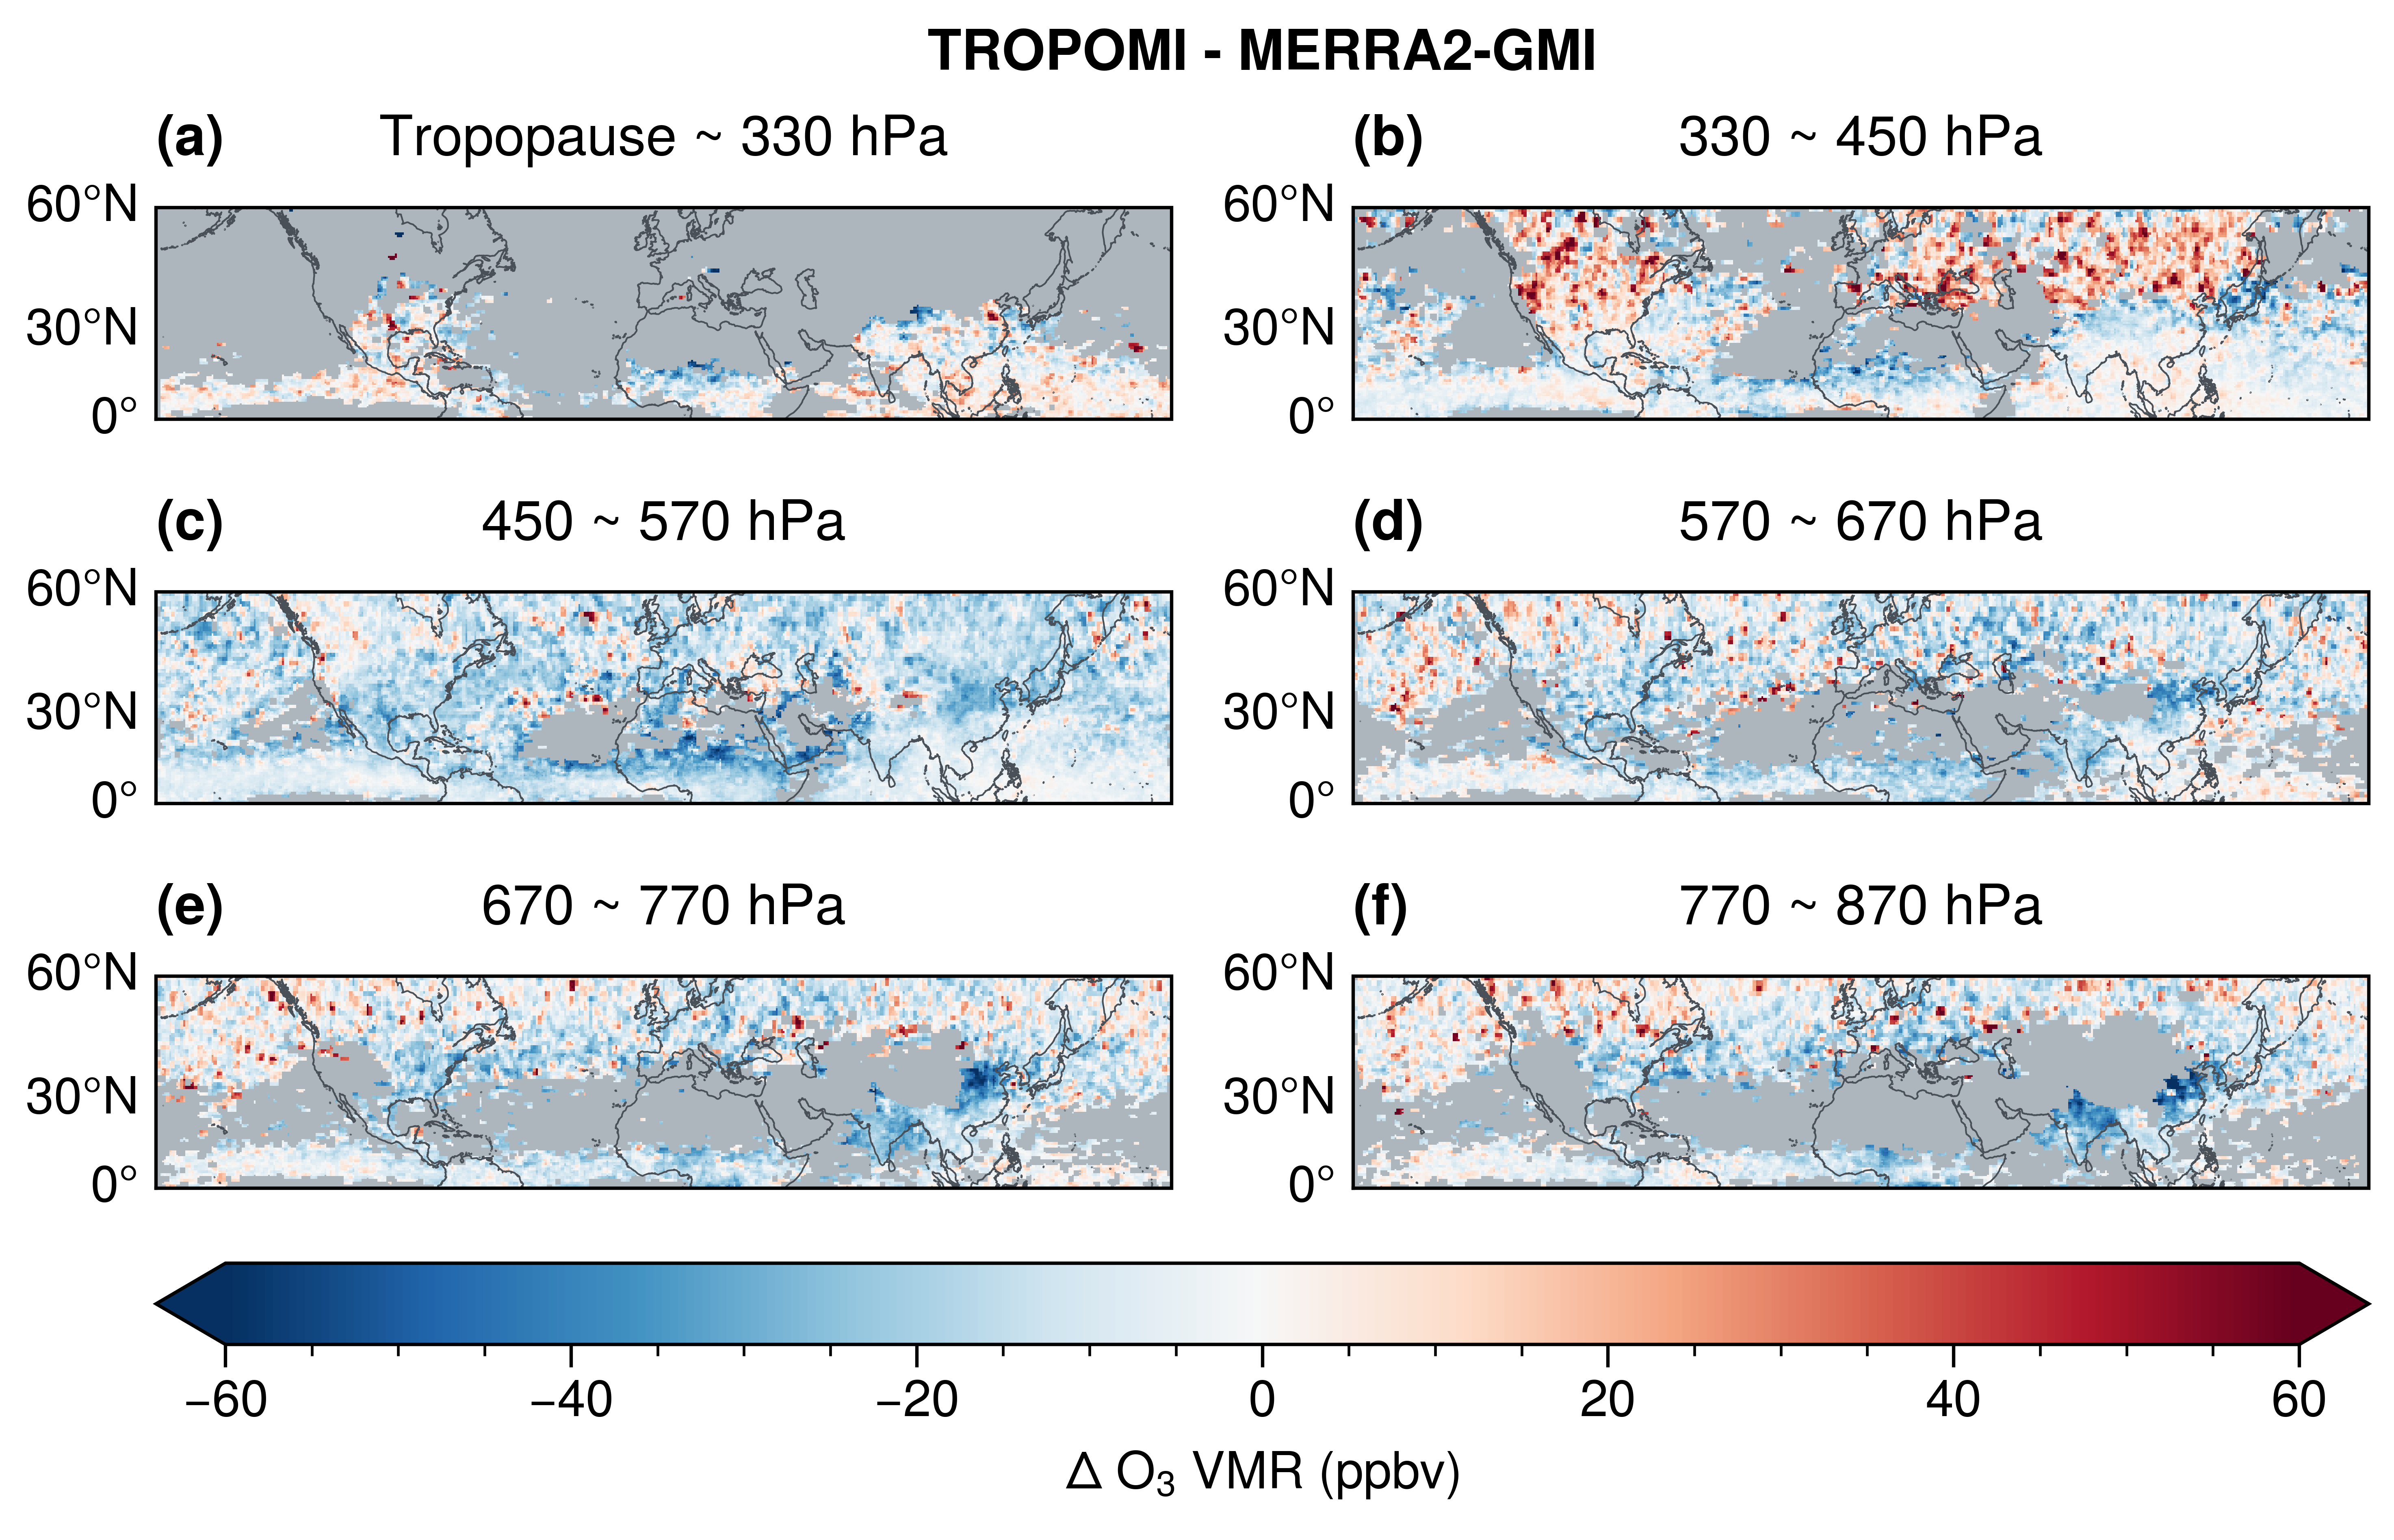
\includegraphics[width=0.9\textwidth]{./figures/uto3_delta.png}
    \caption{
    图\ref{fig:uto3_tropomi}与图\ref{fig:uto3_merra2}之差。 \\
    Figure \ref{fig:uto3_delta}. Differences between Fig. \ref{fig:uto3_tropomi} and Fig. \ref{fig:uto3_merra2}.
    }
    \label{fig:uto3_delta}
\end{figure}


鉴于高云条件下的云切片结果在中纬度地区有效数较少(图\ref{fig:uto3_tropomi}a),
我们将MLS于261 hPa高度观测的O$_{\ch{3}}$浓度与MERRA2-GMI的O$_{\ch{3}}$模拟结果,在晴空和有云条件下分别进行对比。
如图\ref{fig:mls_o3_261hpa}所示,在低纬度地区两者均显示有云条件下海洋上O$_{\ch{3}}$平均浓度较晴空降低17\%,非洲中部和印度北部的O$_{\ch{3}}$平均浓度较晴空增大20\%。
虽然晴空条件下两者在中纬度地区的O$_{\ch{3}}$浓度一致,但有云时两者的变化相反。
具体而言,MLS观测显示有云条件下中纬度地区261 hPa高度的O$_{\ch{3}}$平均浓度比晴空时的浓度高24\%,
而MERRA2-GMI模拟结果显示O$_{\ch{3}}$平均浓度比晴空时低26\%。
在40--60$^{\circ}$ N区域内有高云的条件下,MERRA2-GMI模拟的O$_{\ch{3}}$平均浓度为108 ppbv,与同范围内TROPOMI云切片得到的O$_{\ch{3}}$平均浓度(86 ppbv)相接近,而MLS的平均观测结果(230 ppbv)为MERRA2-GMI和TROPOMI的2--3倍。
由于MLS的O$_{\ch{3}}$廓线在对流层上层的分辨率为3--6 km,而261 hPa所在高度接近中纬度地区的对流层顶,故过度的外推可能导致MLS测得的O$_{\ch{3}}$浓度过高\citep{Schoeberl.2007}。


\begin{figure}[H]
    \centering
    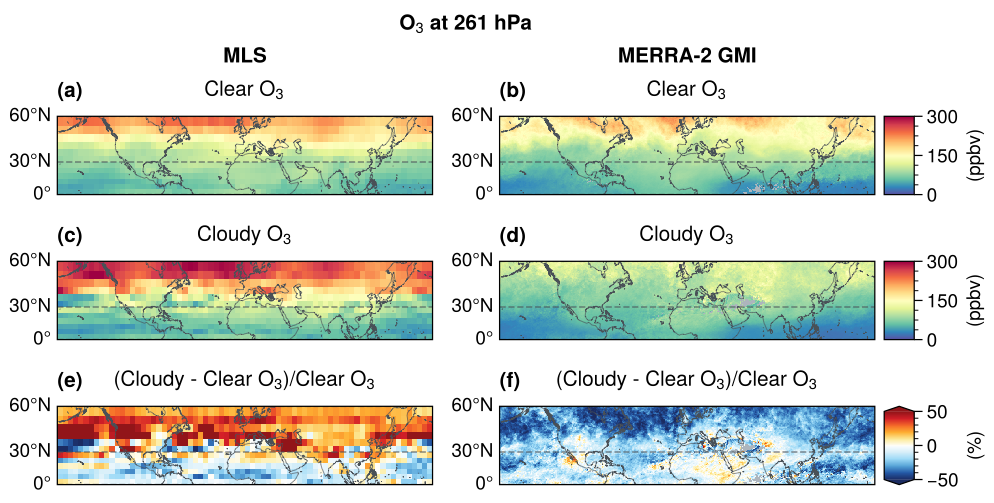
\includegraphics[width=\textwidth]{./figures/mls_o3_261hpa.png}
    \caption{
    2019年6--8月北半球中低纬度晴空(a--b)和有云(c--d)条件下261 hPa高度O$_{\ch{3}}$的平均浓度,以及相对百分比变化(e--f)。
    第一列为MLS观测数据,第二列为MERRA2-GMI模拟结果。 \\
    Figure \ref{fig:mls_o3_261hpa}. The mean O$_{\ch{3}}$ concentrations at 261 hPa with clear (a--b) and cloudy (c--d) conditions at the northern middle-low latitudes for June--August in 2019. The percentage differences are shown in panel (e) and (f).
    The first column is the MLS observations while the second column is the MERRA2-GMI simulations.
    }
    \label{fig:mls_o3_261hpa}
\end{figure}


除了各层O$_{\ch{3}}$浓度的地理分布之外,我们选取了区域内云切片有效层数为6层的格点(位于中国南部、印度中部、美国东南部以及太平洋,图\ref{fig:no2_ltngcount}a),
进行MERRA2-GMI和TROPOMI的廓线对比分析。
如图\ref{fig:uto3_profile}所示,O$_{\ch{3}}$浓度在中云和高云的条件下随着高度升高而降低,
但是由于AMF$_{\ch{geo}}$的限制,低云条件下的O$_{\ch{3}}$浓度在中国南部、印度中部和美国东南部没有显示出O$_{\ch{3}}$的高值,故接下来只比较MERRA2-GMI和TROPOMI在对流层中上层的O$_{\ch{3}}$浓度。
对于中国南部和印度中部,MERRA2-GMI的模拟值高于TROPOMI的观测值,两者之差从570--670 hPa的20 pptv逐渐下降至对流层顶--330 hPa的2 pptv。
对于美国东南部,TROPOMI的观测值在330--450 hPa间有一峰值,与图\ref{fig:utno2_profile}c中LNO$_{\ch{2}}$峰值相对应,
而MERRA2-GMI的模拟结果在该高度不存在O$_{\ch{3}}$峰值,即MERRA2-GMI对流层上层LNO$_{\ch{2}}$的差异导致O$_{\ch{3}}$的低估。
对于清洁的太平洋地区,两者随高度而降低的趋势一致,且误差小于5 pptv。
总之,TROPOMI的观测结果和MERRA2-GMI的模拟结果在对流层中上层存在显著的一致性,
局部的差异表明云切片方法可以用来检验模式中LNO$_{\ch{x}}$的产量和影响。


\begin{figure}[H]
    \centering
    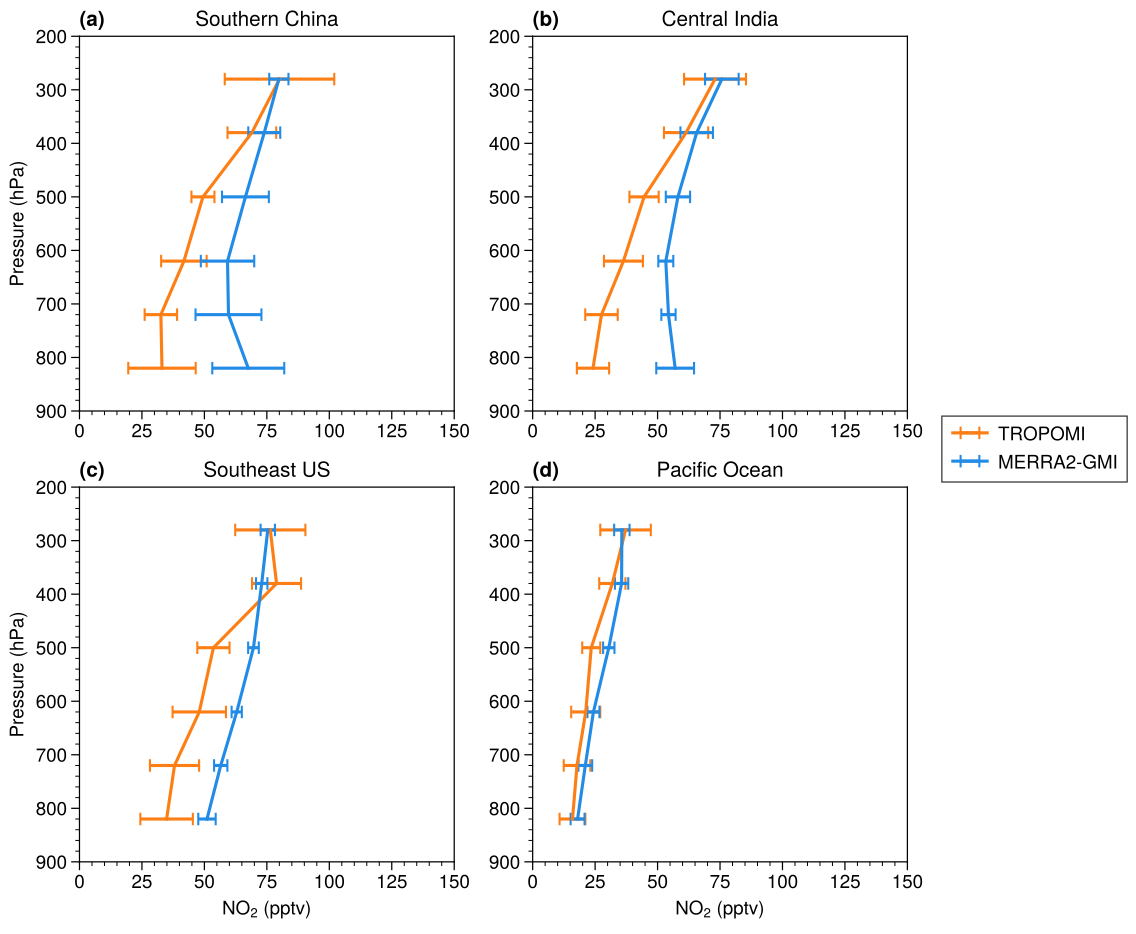
\includegraphics[width=0.9\textwidth]{./figures/uto3_profile.png}
    \caption{
    MERRA2-GMI(蓝色)和TROPOMI云切片算法(橙色)得到的区域平均O$_{\ch{3}}$廓线
    (a)中国南部;(b)印度中部;(c)美国东南部;(d)太平洋(区域示意图见图\ref{fig:no2_ltngcount}a)。
    其中廓线的误差棒为平均值$\pm$标准差。\\
    Figure \ref{fig:uto3_profile}. Regional average NO$_{\ch{2}}$ profiles obtained by MERRA2-GMI (blue) and TROPOMI cloud slice algorithm (orange).
    (a) southern China, (b) central India, (c) southeastern United States, and (d) Pacific Ocean
    (Definitions of region are shown in Fig. \ref{fig:no2_ltngcount}a).
    The error bars are the mean values $\pm$ standard deviations.
    }
    \label{fig:uto3_profile}
\end{figure}

\begin{figure}[H]
\centering
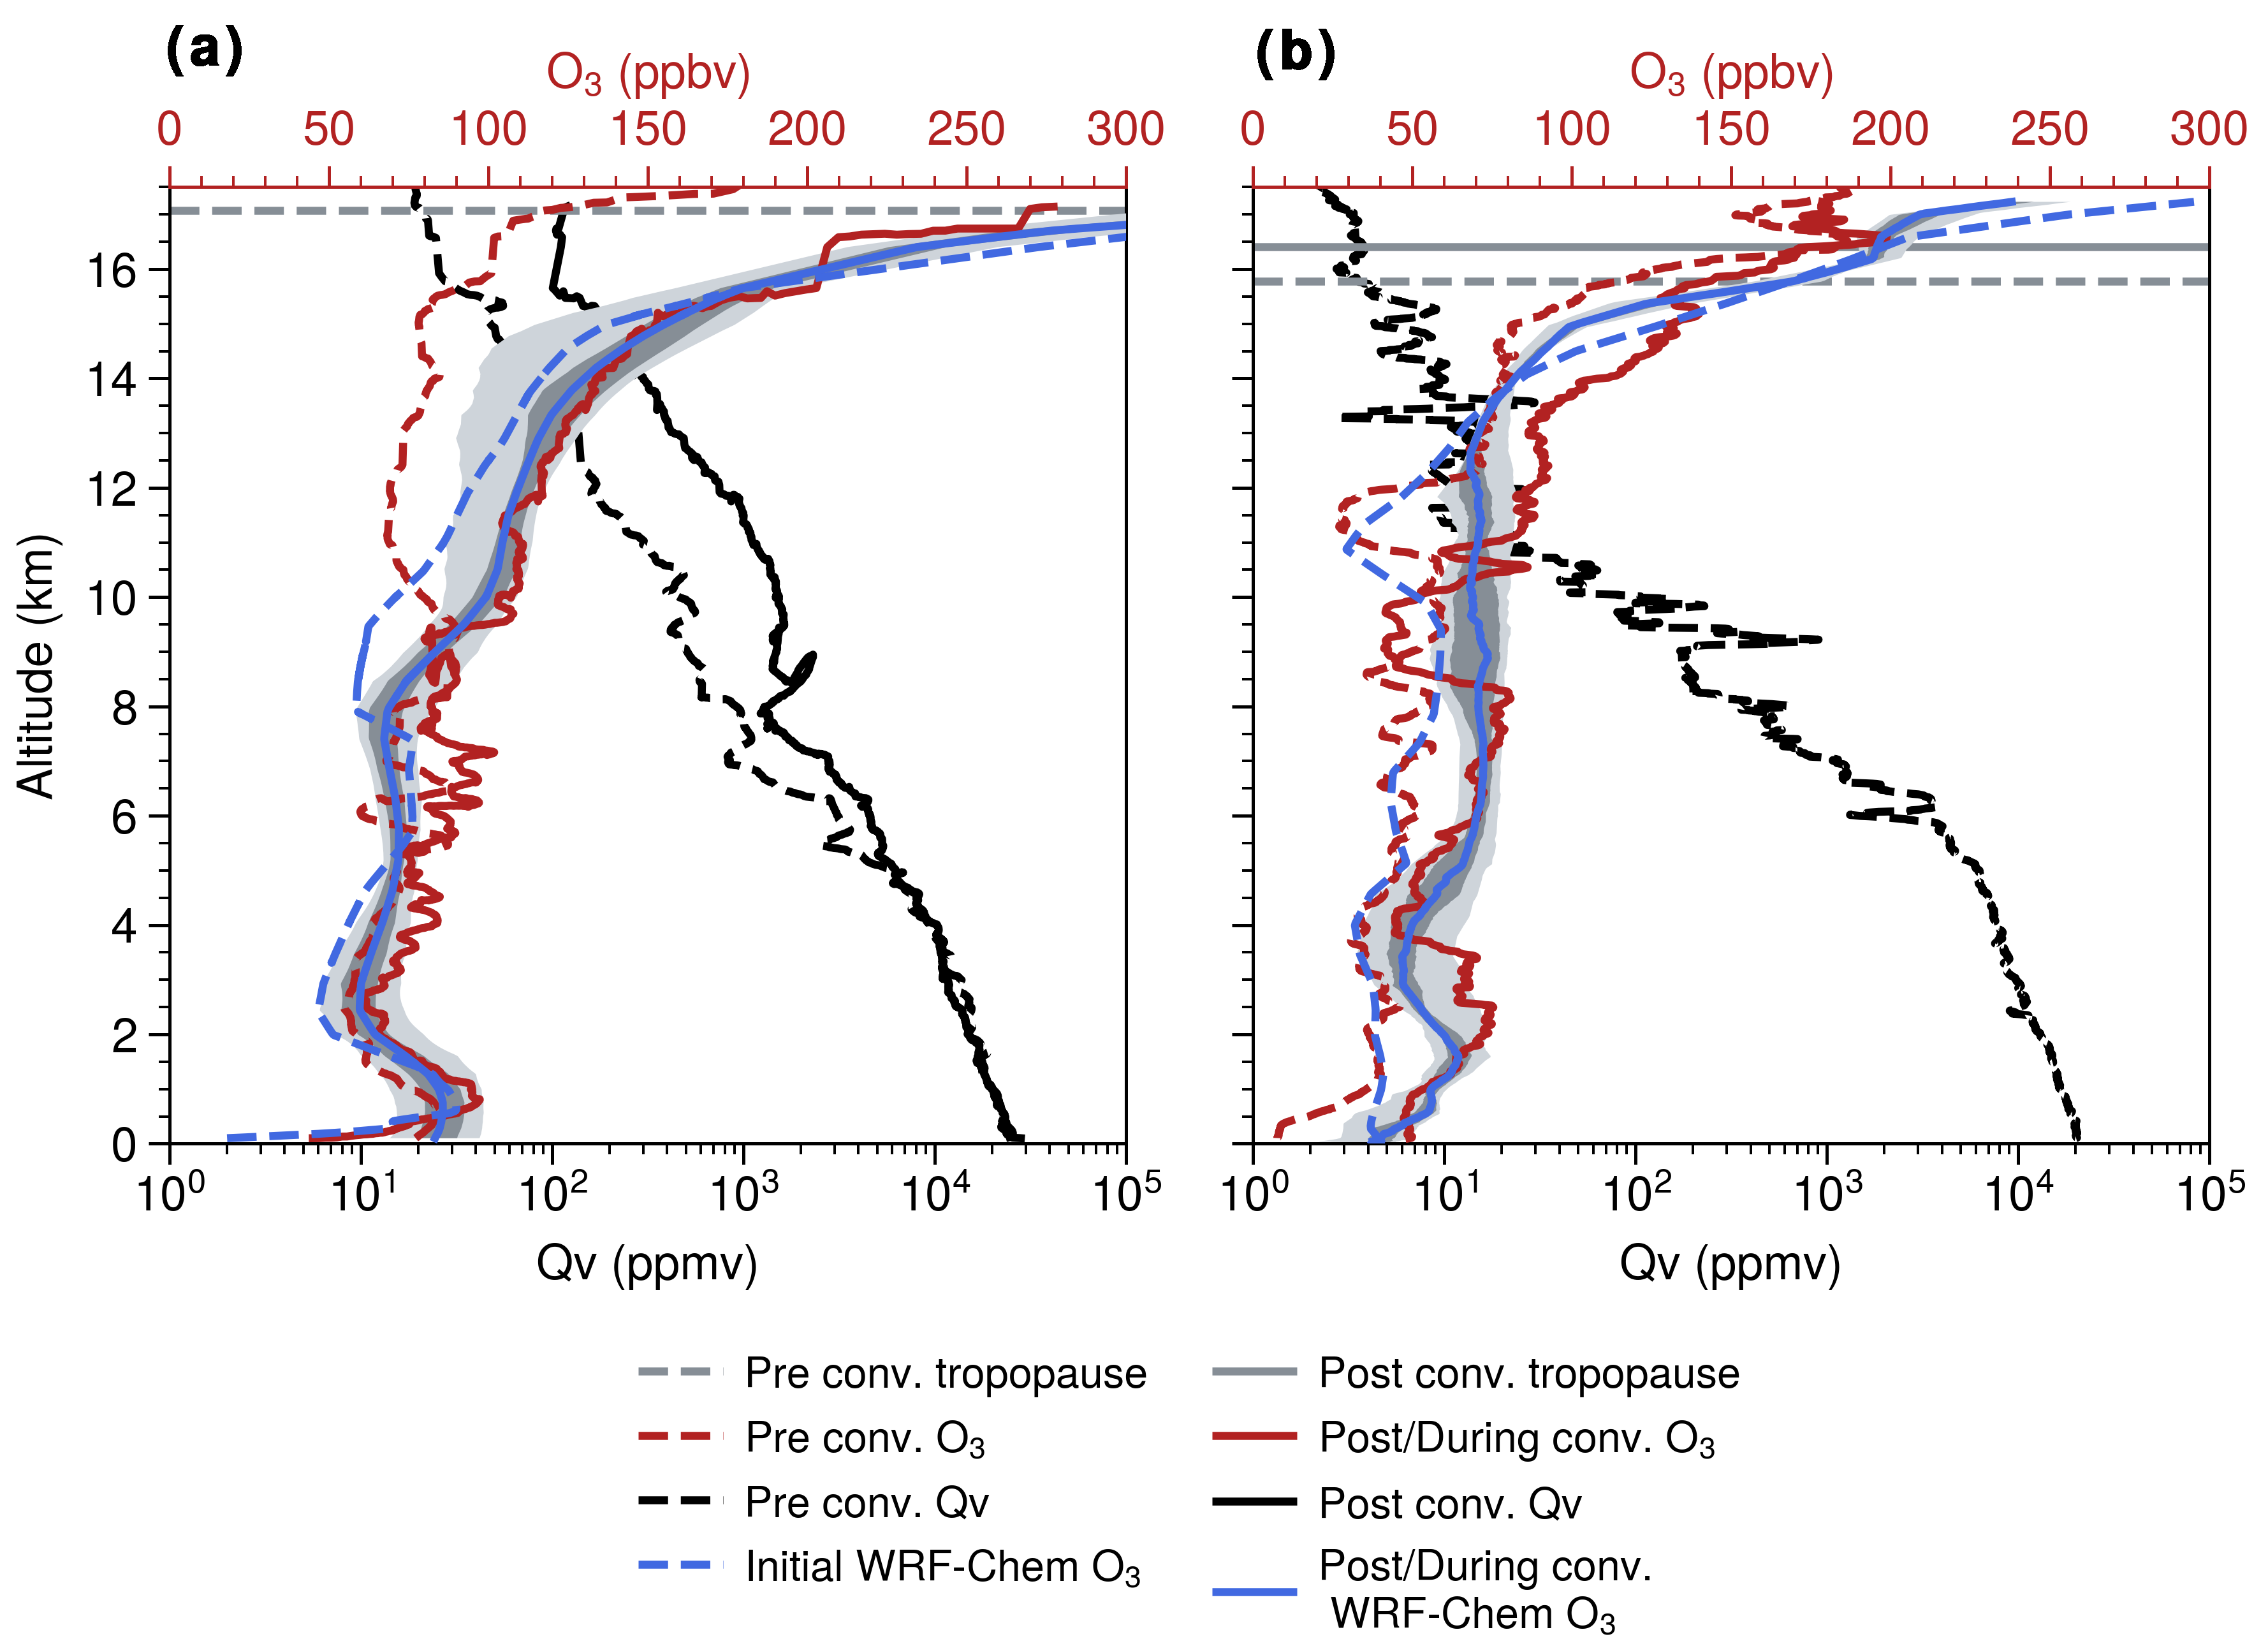
\includegraphics[width=0.9\textwidth]{./figures/ozonesonde_profile.png}
\caption{对流前(虚线)和对流后/对流期间(实线)探空观测到的O$_{\ch{3}}$(红色)和Q$_v$(黑色)廓线。
模式初始(虚线)和对流后或对流期间(实线)的O$_{\ch{3}}$廓线为蓝色。
深灰色阴影是50\%的置信区间,浅色是90\%的置信区间,灰线是第一对流层顶。
(a)2019年个例;(b)2020年个例。\\
Figure \ref{fig:ozonesonde_profile}. Observed O$_{\ch{3}}$ (red) and Q$_v$ (black) profiles in the pre-convection (dashed) and post-convection/during-convection (solid) periods.
The initial (dashed) and simulated post-convection or during-convection (solid) O$_{\ch{3}}$ profiles are in blue.
The dark gray shading is the 50 \% confidence interval while the light one is the 90 \% confidence interval.
The gray lines are the lapse rate tropopauses.
(a) 2019 case and (b) 2020 case.
}
\label{fig:ozonesonde_profile}
\end{figure}

除了云切片算法得到的全球O$_{\ch{3}}$分布外,
中国东南部的臭氧探空试验在对流不同阶段所测得的O$_{\ch{3}}$和Q$_v$分布如图\ref{fig:ozonesonde_profile}所示。
总体来说,对流导致对流层上层O$_{\ch{3}}$和Q$_v$浓度增大,且增强的最大值所在区域居于10--16 km 之间。
% 其中2020年个例的对流层低层(2--8 km)O$_{\ch{3}}$浓度有较大的增加。
两个个例均存在双谷形的O$_{\ch{3}}$廓线,但高度不同:2019年的热对流个例为2 和8 km,2020年的飑线为4 和10 km。
尽管WRF-Chem模式倾向于低估2019年个例对流层下层和2020年个例对流层上层中的O$_{\ch{3}}$浓度,
但仍再现了详细的O$_{\ch{3}}$垂直分布,故能用以分析对流影响O$_{\ch{3}}$的机制。
其中共有三个来源可以解释对流层上层O$_{\ch{3}}$的增加:对流输送、化学反应和闪电直接产生的O$_{\ch{3}}$。
\ref{sec:convec_impacts}节仅详细讨论前两个因素,因为闪电直接产生的O$_{\ch{3}}$
产量仍不确定\citep{Morris.2010,Ripoll.2014}.

\section{臭氧浓度变化的原因}

\subsection{动力输送和化学反应的贡献} \label{sec:convec_impacts}

为了探究中国东南部对流后对流层上层O$_{\ch{3}}$浓度增大的原因,我们将对流分为三个阶段(初生、发展和消散)来分析臭氧探空仪所经区域中O$_{\ch{3}}$平均浓度的垂直分布廓线变化(图\ref{fig:tendency_o3}a,d)。
其中,2020年个例的对流层上层O$_{\ch{3}}$在整个周期内一直在增加,而2019年个例由于发展阶段低浓度O$_{\ch{3}}$空气的抬升,O$_{\ch{3}}$浓度降低,接着又开始增大,这种现象可以用发展阶段的O$_{\ch{3}}$垂直剖面来解释(图\ref{fig:tendency_o3}b),
低O$_{\ch{3}}$浓度的空气块通过上升气流达到16 km,然后对流后方的高O$_{\ch{3}}$浓度空气被夹卷进该区域。
而2020年个例中观测到增加的O$_{\ch{3}}$,主要来自垂直传输的背景O$_{\ch{3}}$浓度(图\ref{fig:tendency_o3}e)。

为了确定两种影响之间的差异,我们分析了对流期间10--14 km的平均累积物理变化速率(IPR,图\ref{fig:tendency_o3}c,f)。
其中水平平流(advh)和垂直平流(advz)的相反趋势支配着2019年对流层上层O$_{\ch{3}}$产率的下降。
由于强上升气流使得低O$_{\ch{3}}$浓度的空气块得以抬升,故垂直平流(advz)的贡献在10--11.5 km之间为负,而在11.5到13.8km 之间为正,即存在向下输送的高浓度O$_{\ch{3}}$空气块。
由于2020年对流个例发生后的Q$_v$较高(图\ref{fig:ozonesonde_profile}a)且对流层顶高于云区(图\ref{fig:tendency_o3}b),
所以其上升气流不足以像中尺度对流系统一样将平流层高浓度的O$_{\ch{3}}$挟至对流层\citep{Phoenix.2020}。
虽然动力输送在O$_{\ch{3}}$的变化中起着重要作用,但不能忽视正的化学贡献,尤其是2020年对流期间化学贡献造成对流层上层O$_{\ch{3}}$的净增加。
具体来说,在两次个例整个生命期中化学反应对O$_{\ch{3}}$起到了正贡献,
其影响程度是动力输送的5--10倍,这表明化学贡献在对流的整个生命期中占主导地位。


\begin{figure}[H]
\centering
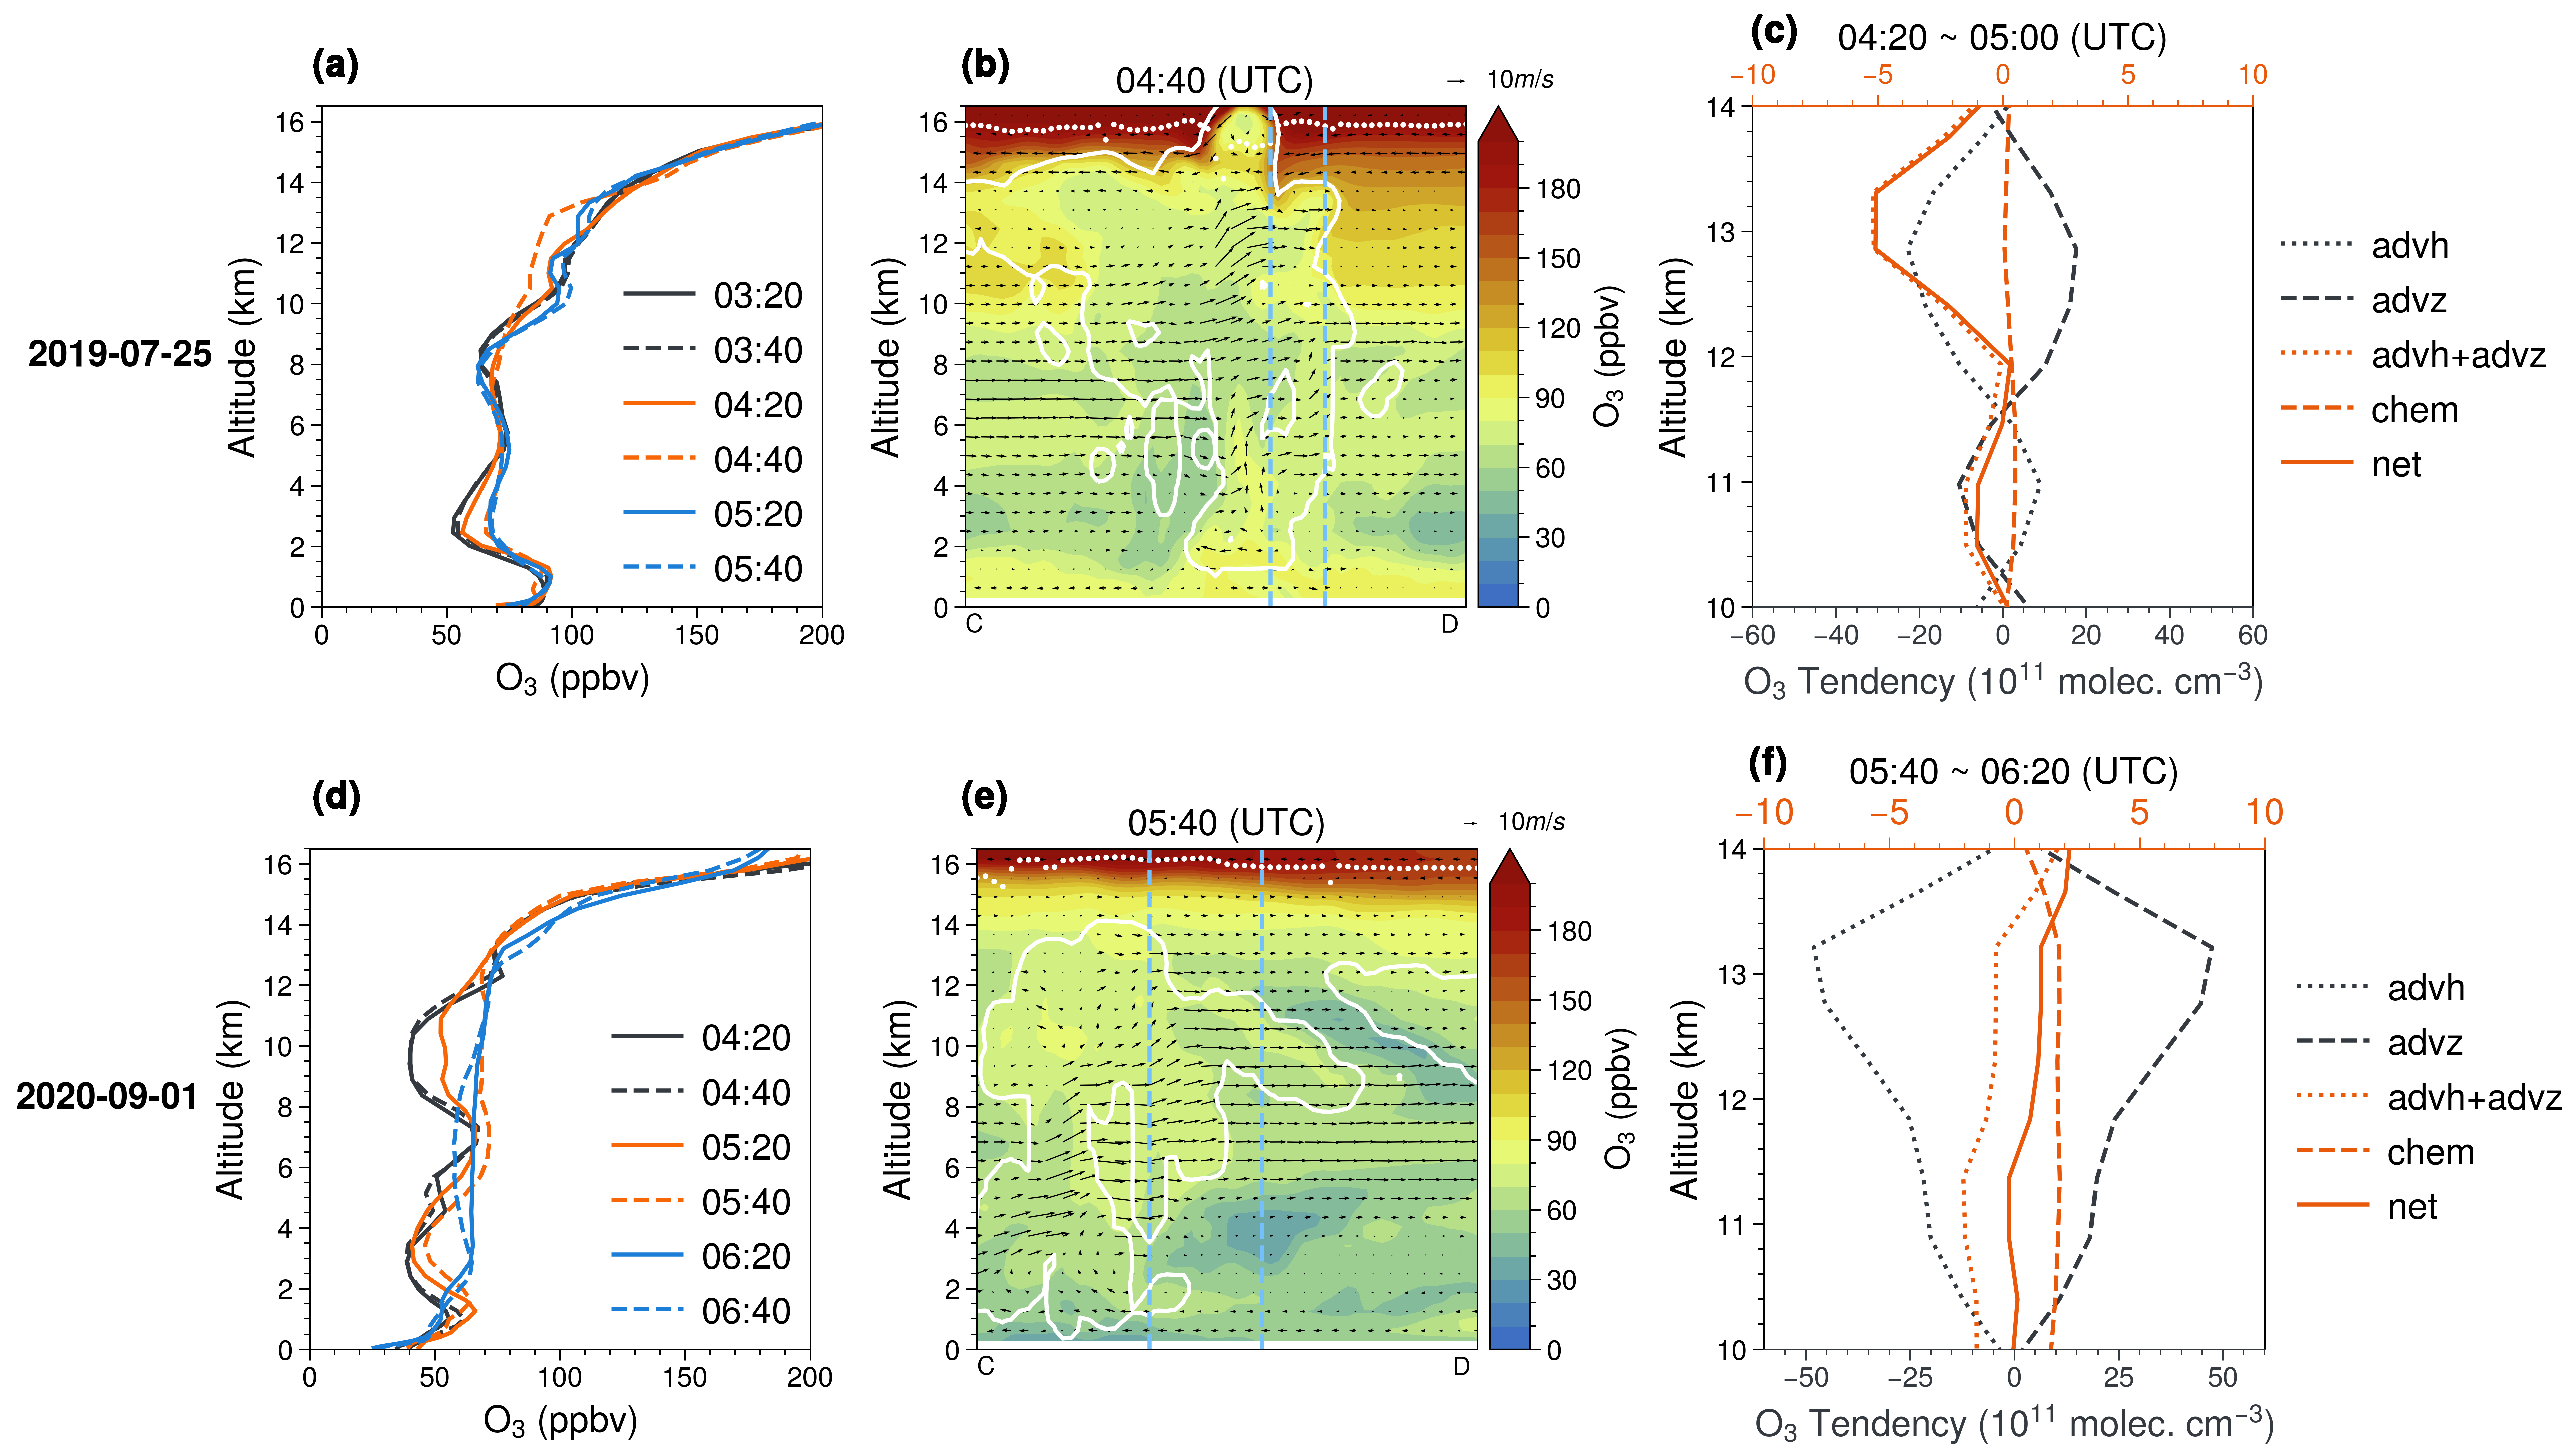
\includegraphics[width=\textwidth]{./figures/tendency_o3.png}
\caption{
(a, d)臭氧探空仪所经区域内的O$_{\ch{3}}$平均浓度剖面,包括三个阶段:初生(黑色)、发展(橙色)和消散(蓝色);
(b,e)对流旺盛期间沿穿过对流核心(图 \ref{fig:comp_crf_2019}e 和图 \ref{fig:comp_crf_2020}f)的O$_{\ch{3}}$剖面。
蓝色虚线代表臭氧探空仪经过区域的边界,第一对流层顶显示为白点。
白线为云边界[云液态水混合比(q$_{cloud}$)和冰混合比(q$_{ice}$)之和 $\geq$ 0.01 g/kg];
(c, f)对流旺盛期间水平平流(advh)、垂直平流(advz)和化学贡献(chem)在臭氧探空仪所经区域内导致的O$_{\ch{3}}$净产率的垂直分布。
\\
Figure \ref{fig:tendency_o3}. (a, d) The mean O$_{\ch{3}}$ profiles in the regions passed by the ozonesondes
at three stages: initiation (black), development (orange), and dissipation (blue).
(b, e) Vertical O$_{\ch{3}}$ distribution within the convective periods along the line crossing the convective core (Fig. \ref{fig:comp_crf_2019}e and Fig. \ref{fig:comp_crf_2020}f).
The blue dashed lines stand for the boundaries of regions passed by the ozonesondes, and the lapse rate tropopause is shown as the white dots.
The cloud boundaries [the sum of cloud liquid water mixing ratio (q$_{cloud}$) and ice mixing ratio (q$_{ice}$) $\geq$ 0.01 g/kg] are shown in white lines.
(c, f) The vertical distributions of the O$_{\ch{3}}$ net production rate and tendency due to horizontal advection (advh), vertical advection (advz), and chemistry (chem) during the convective periods.
}
\label{fig:tendency_o3}
\end{figure}


除臭氧探空所经的固定区域之外,我们也将对流分为对流核心区(组合雷达反射率$\geq$40 dBZ)和层云区(10 dBZ$\leq$组合雷达反射率$<$40 dBZ)
来探讨旺盛期间对流不同部位的O$_3$浓度变化及其原因,
对流分区的详细示意图如图\ref{fig:china_classification_2019}和图\ref{fig:china_classification_2020}所示。
由于臭氧探空仪所经区域为对流旺盛区,所以与图\ref{fig:tendency_o3}e和f相符,在对流核心区域内,2019年个例动力输送造成的负贡献占主导,2020年个例化学正贡献占主导。
然而层云区域内两个个例的O$_3$浓度变化均为动力输送占主导,
且O$_3$变化的垂直分布与对流核心区相似,
即动力输送可将对流核心区的O$_3$输送至外围层云区,从而导致层云区域内O$_3$浓度呈现类似的变化。

\begin{figure}[H]
\centering
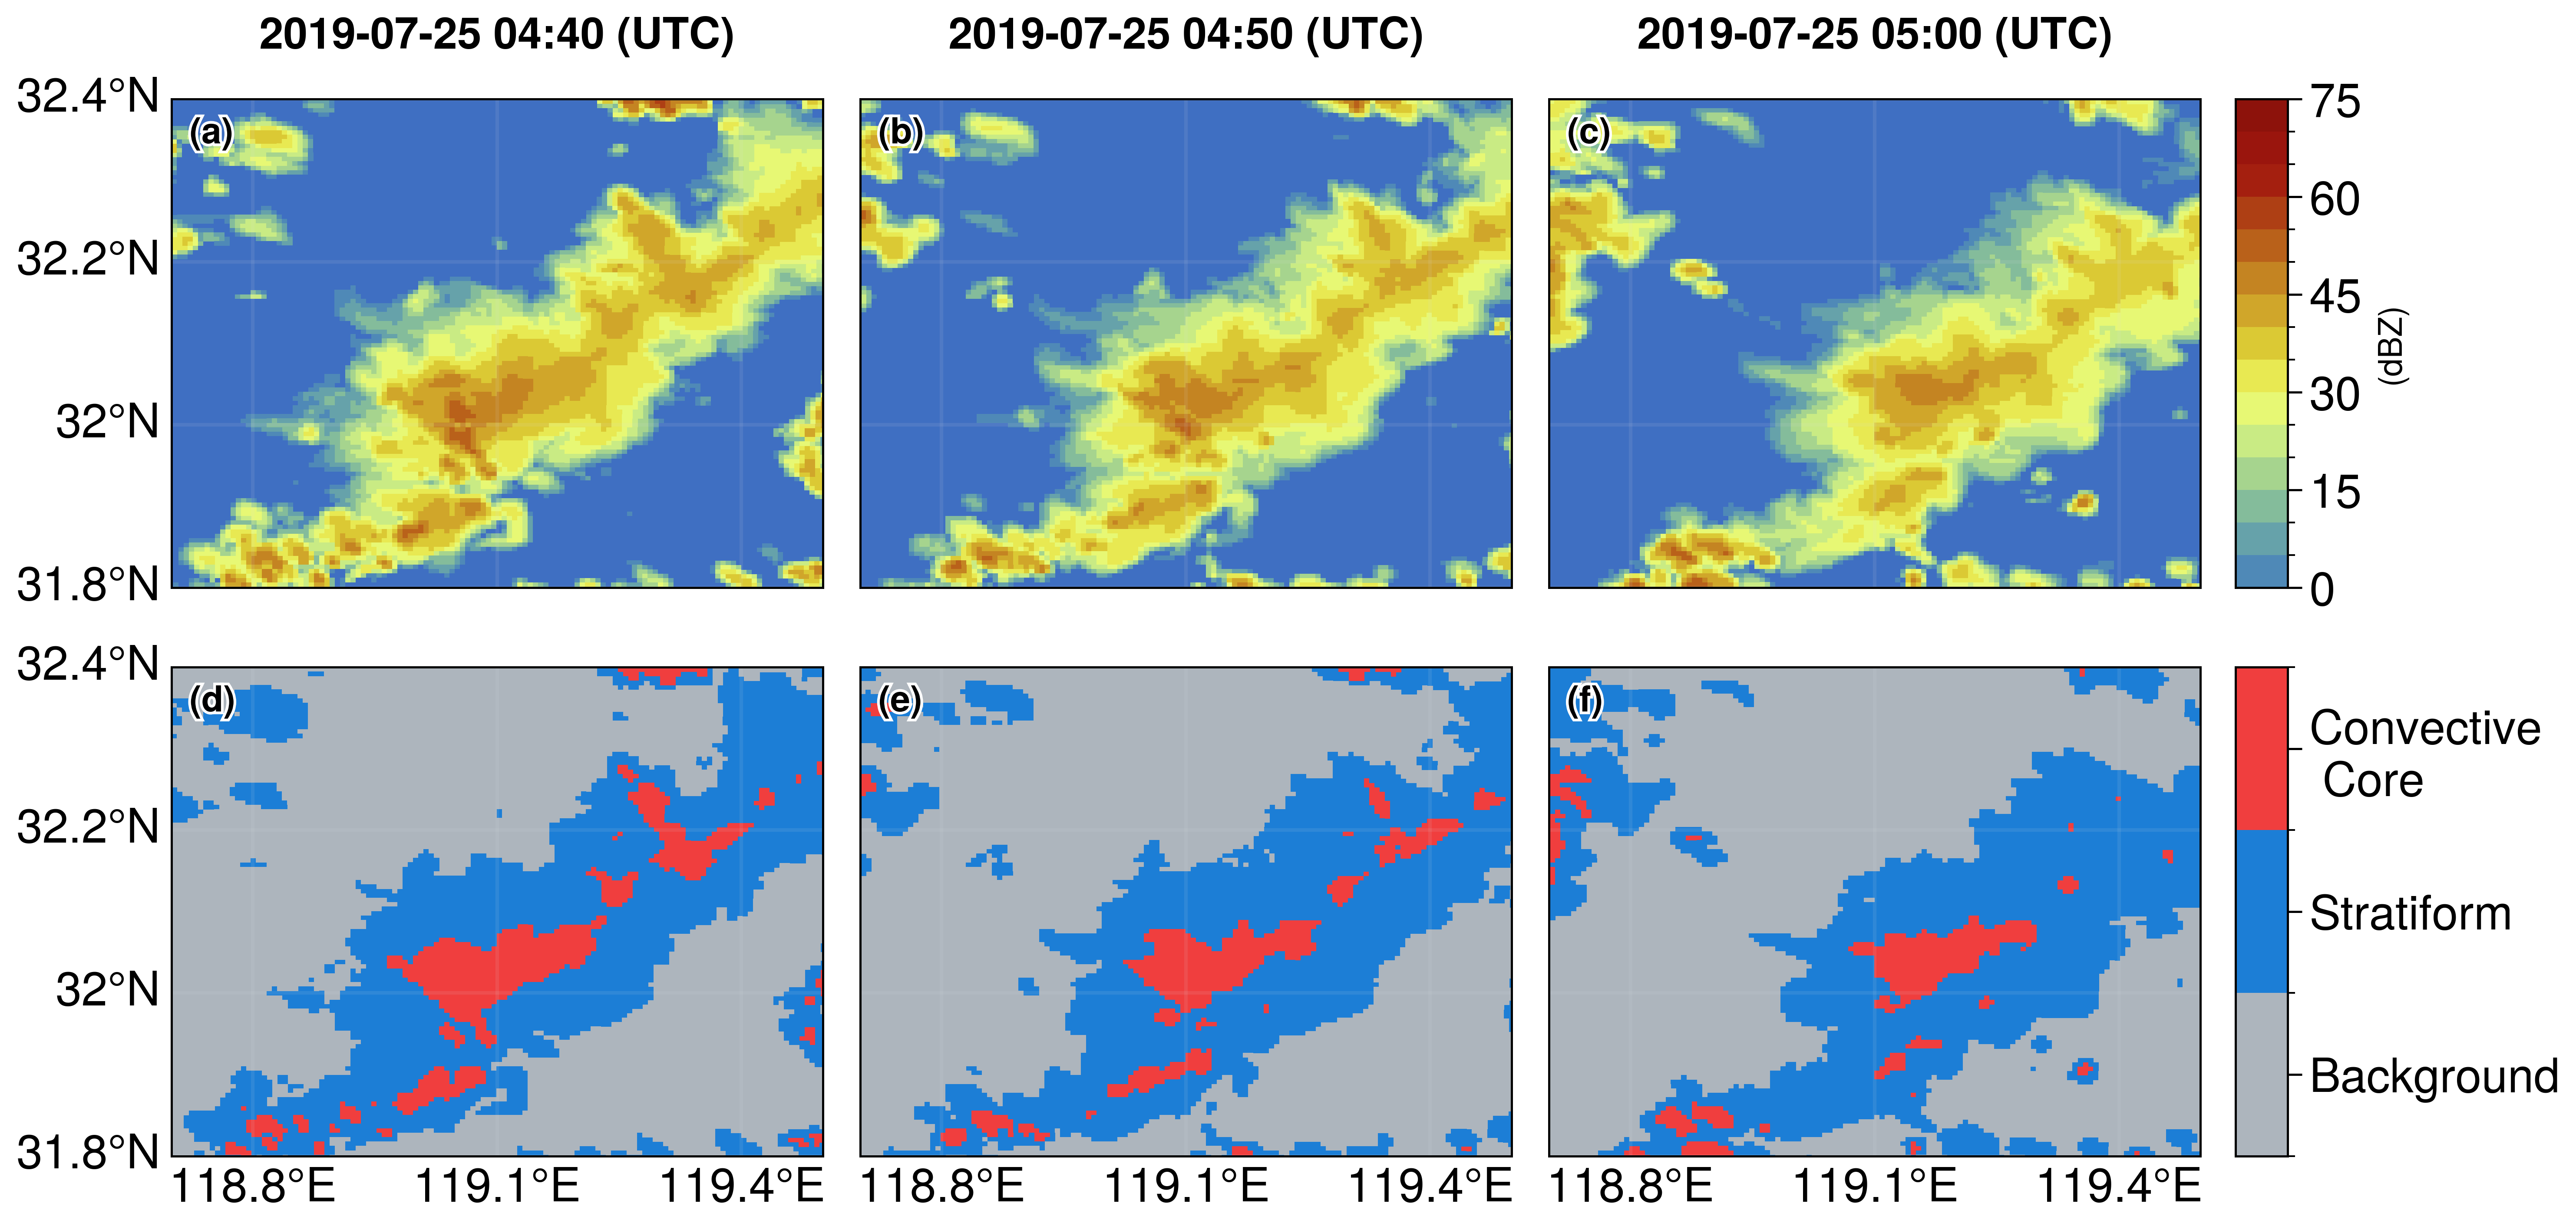
\includegraphics[width=\textwidth]{./figures/china_classification_2019.png}
\caption{
2019年个例对流旺盛期间
(a--c)观测的组合雷达反射率,
(d--f)对流核心区和层云区的定义。\\
Figure \ref{fig:china_classification_2019}.
(a--c) Observed radar composite reflectivity,
(d--f) definitions of convective and stratiform regions during the convective periods of 2019 case.
}
\label{fig:china_classification_2019}
\end{figure}

\begin{figure}[H]
\centering
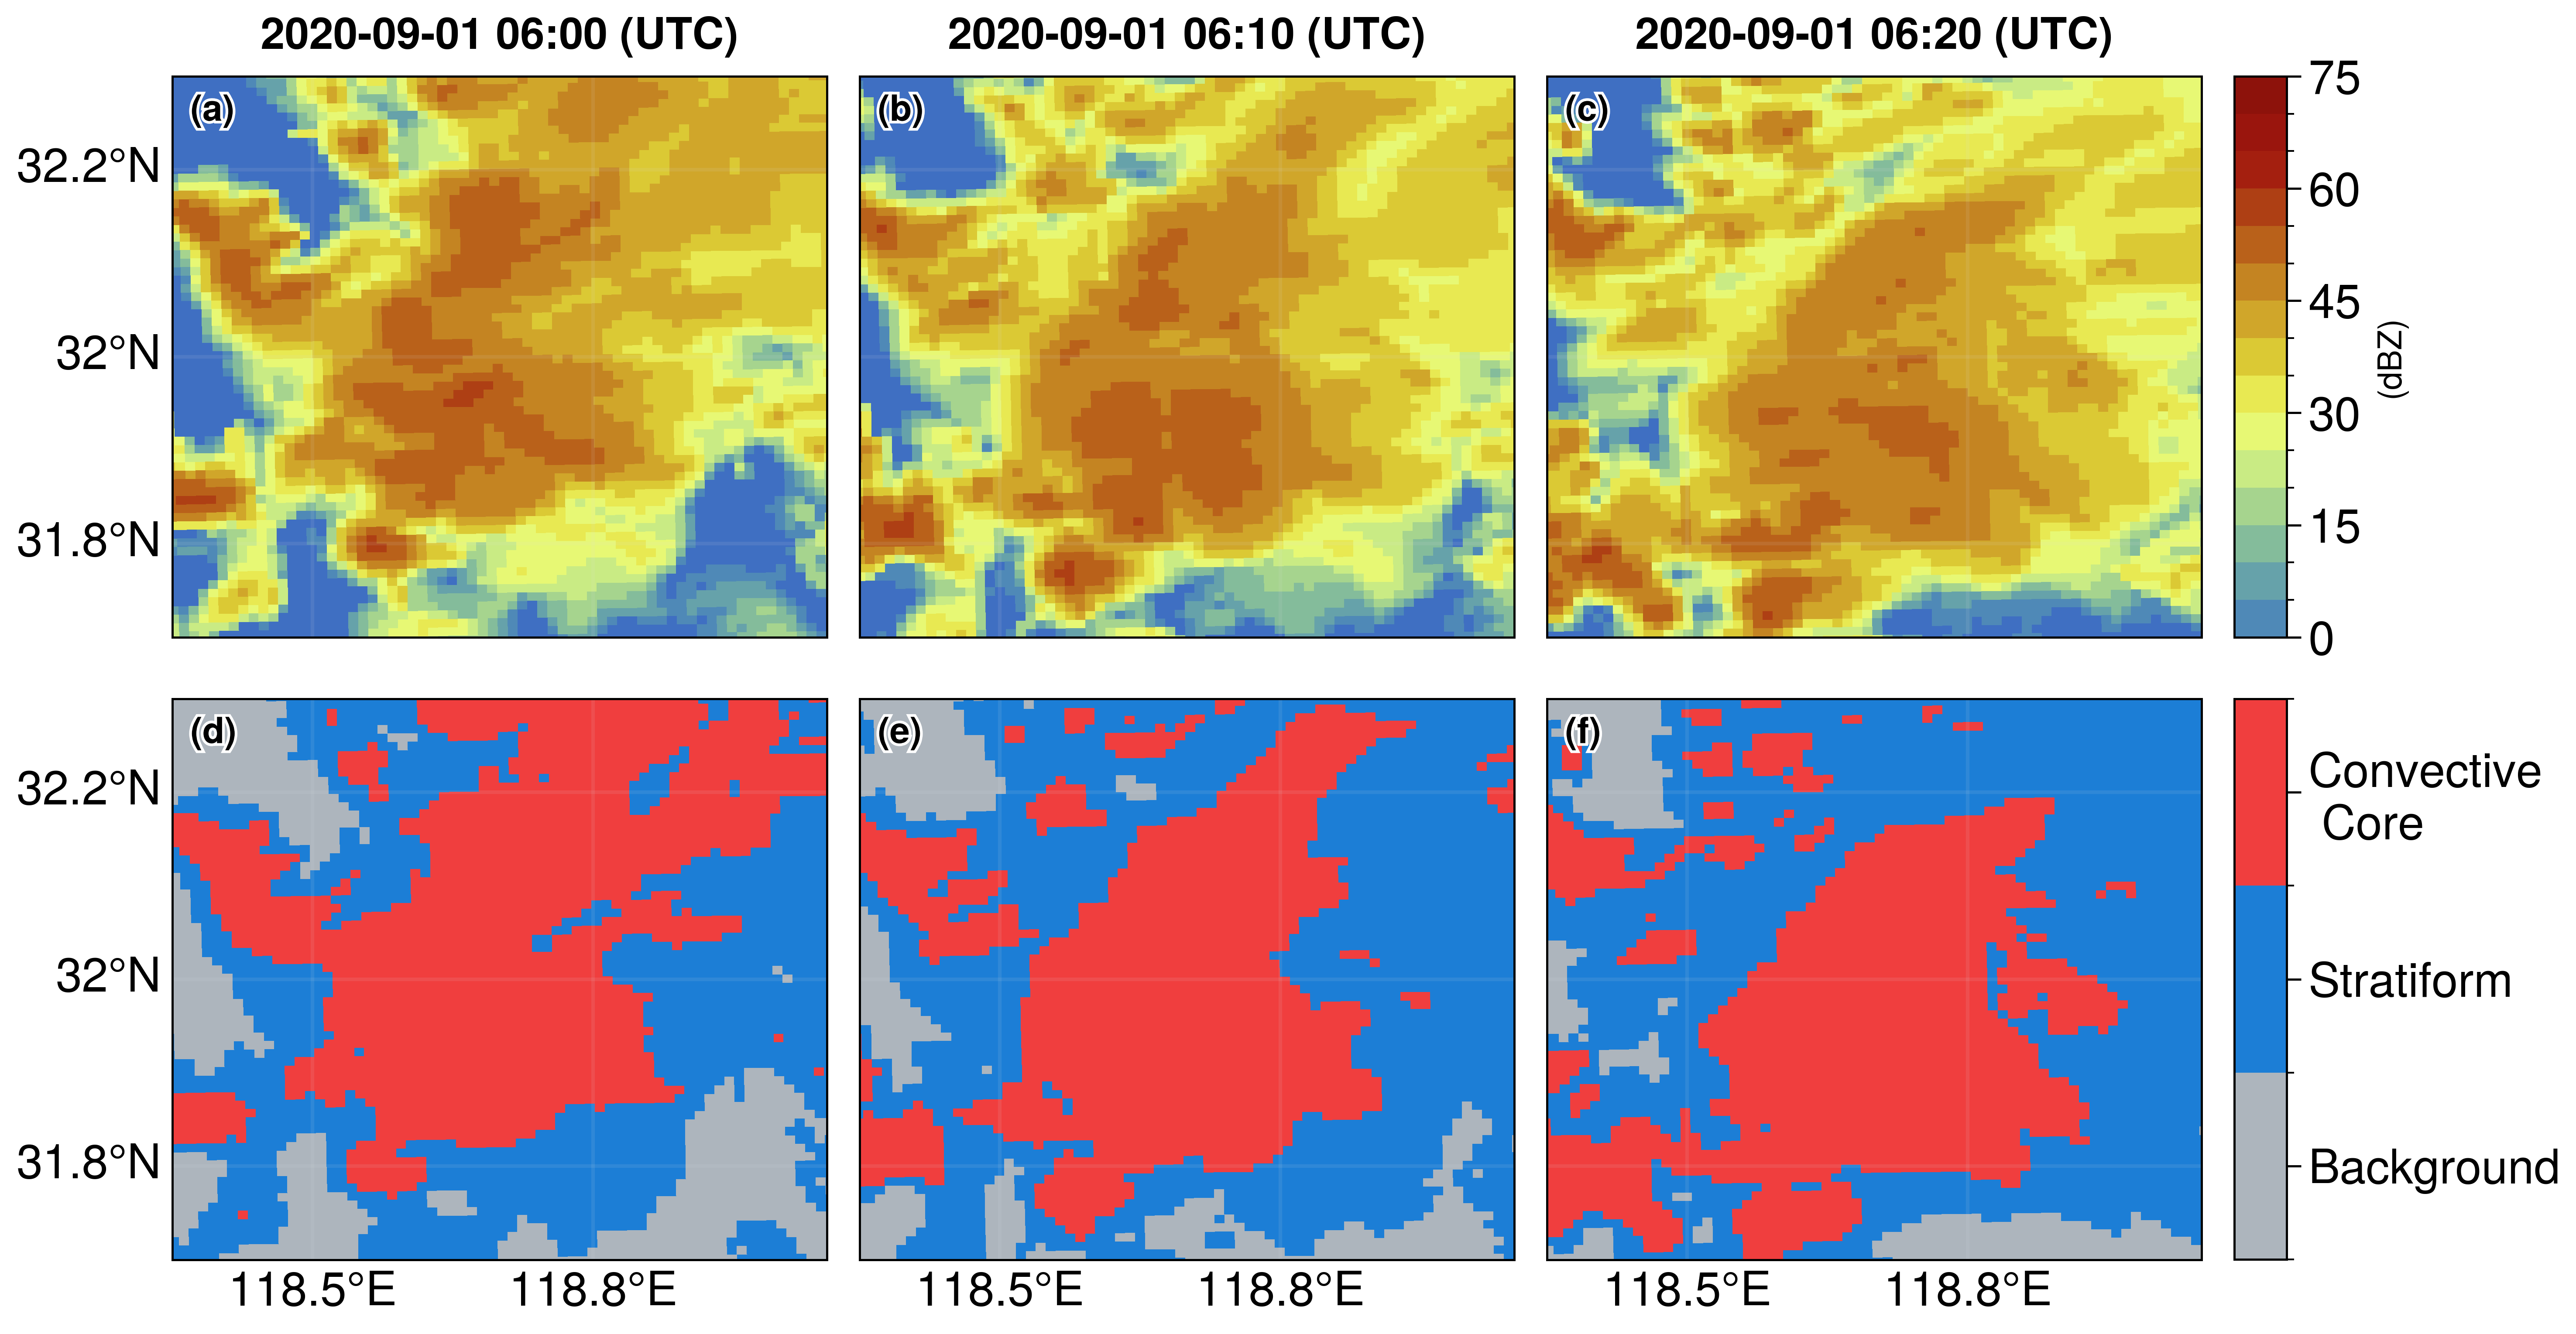
\includegraphics[width=0.95\textwidth]{./figures/china_classification_2020.png}
\caption{
同图\ref{fig:china_classification_2019},但为2020年个例。\\
Same as Fig. \ref{fig:china_classification_2019} but for the 2020 case.
}
\label{fig:china_classification_2020}
\end{figure}

\begin{figure}[H]
\centering
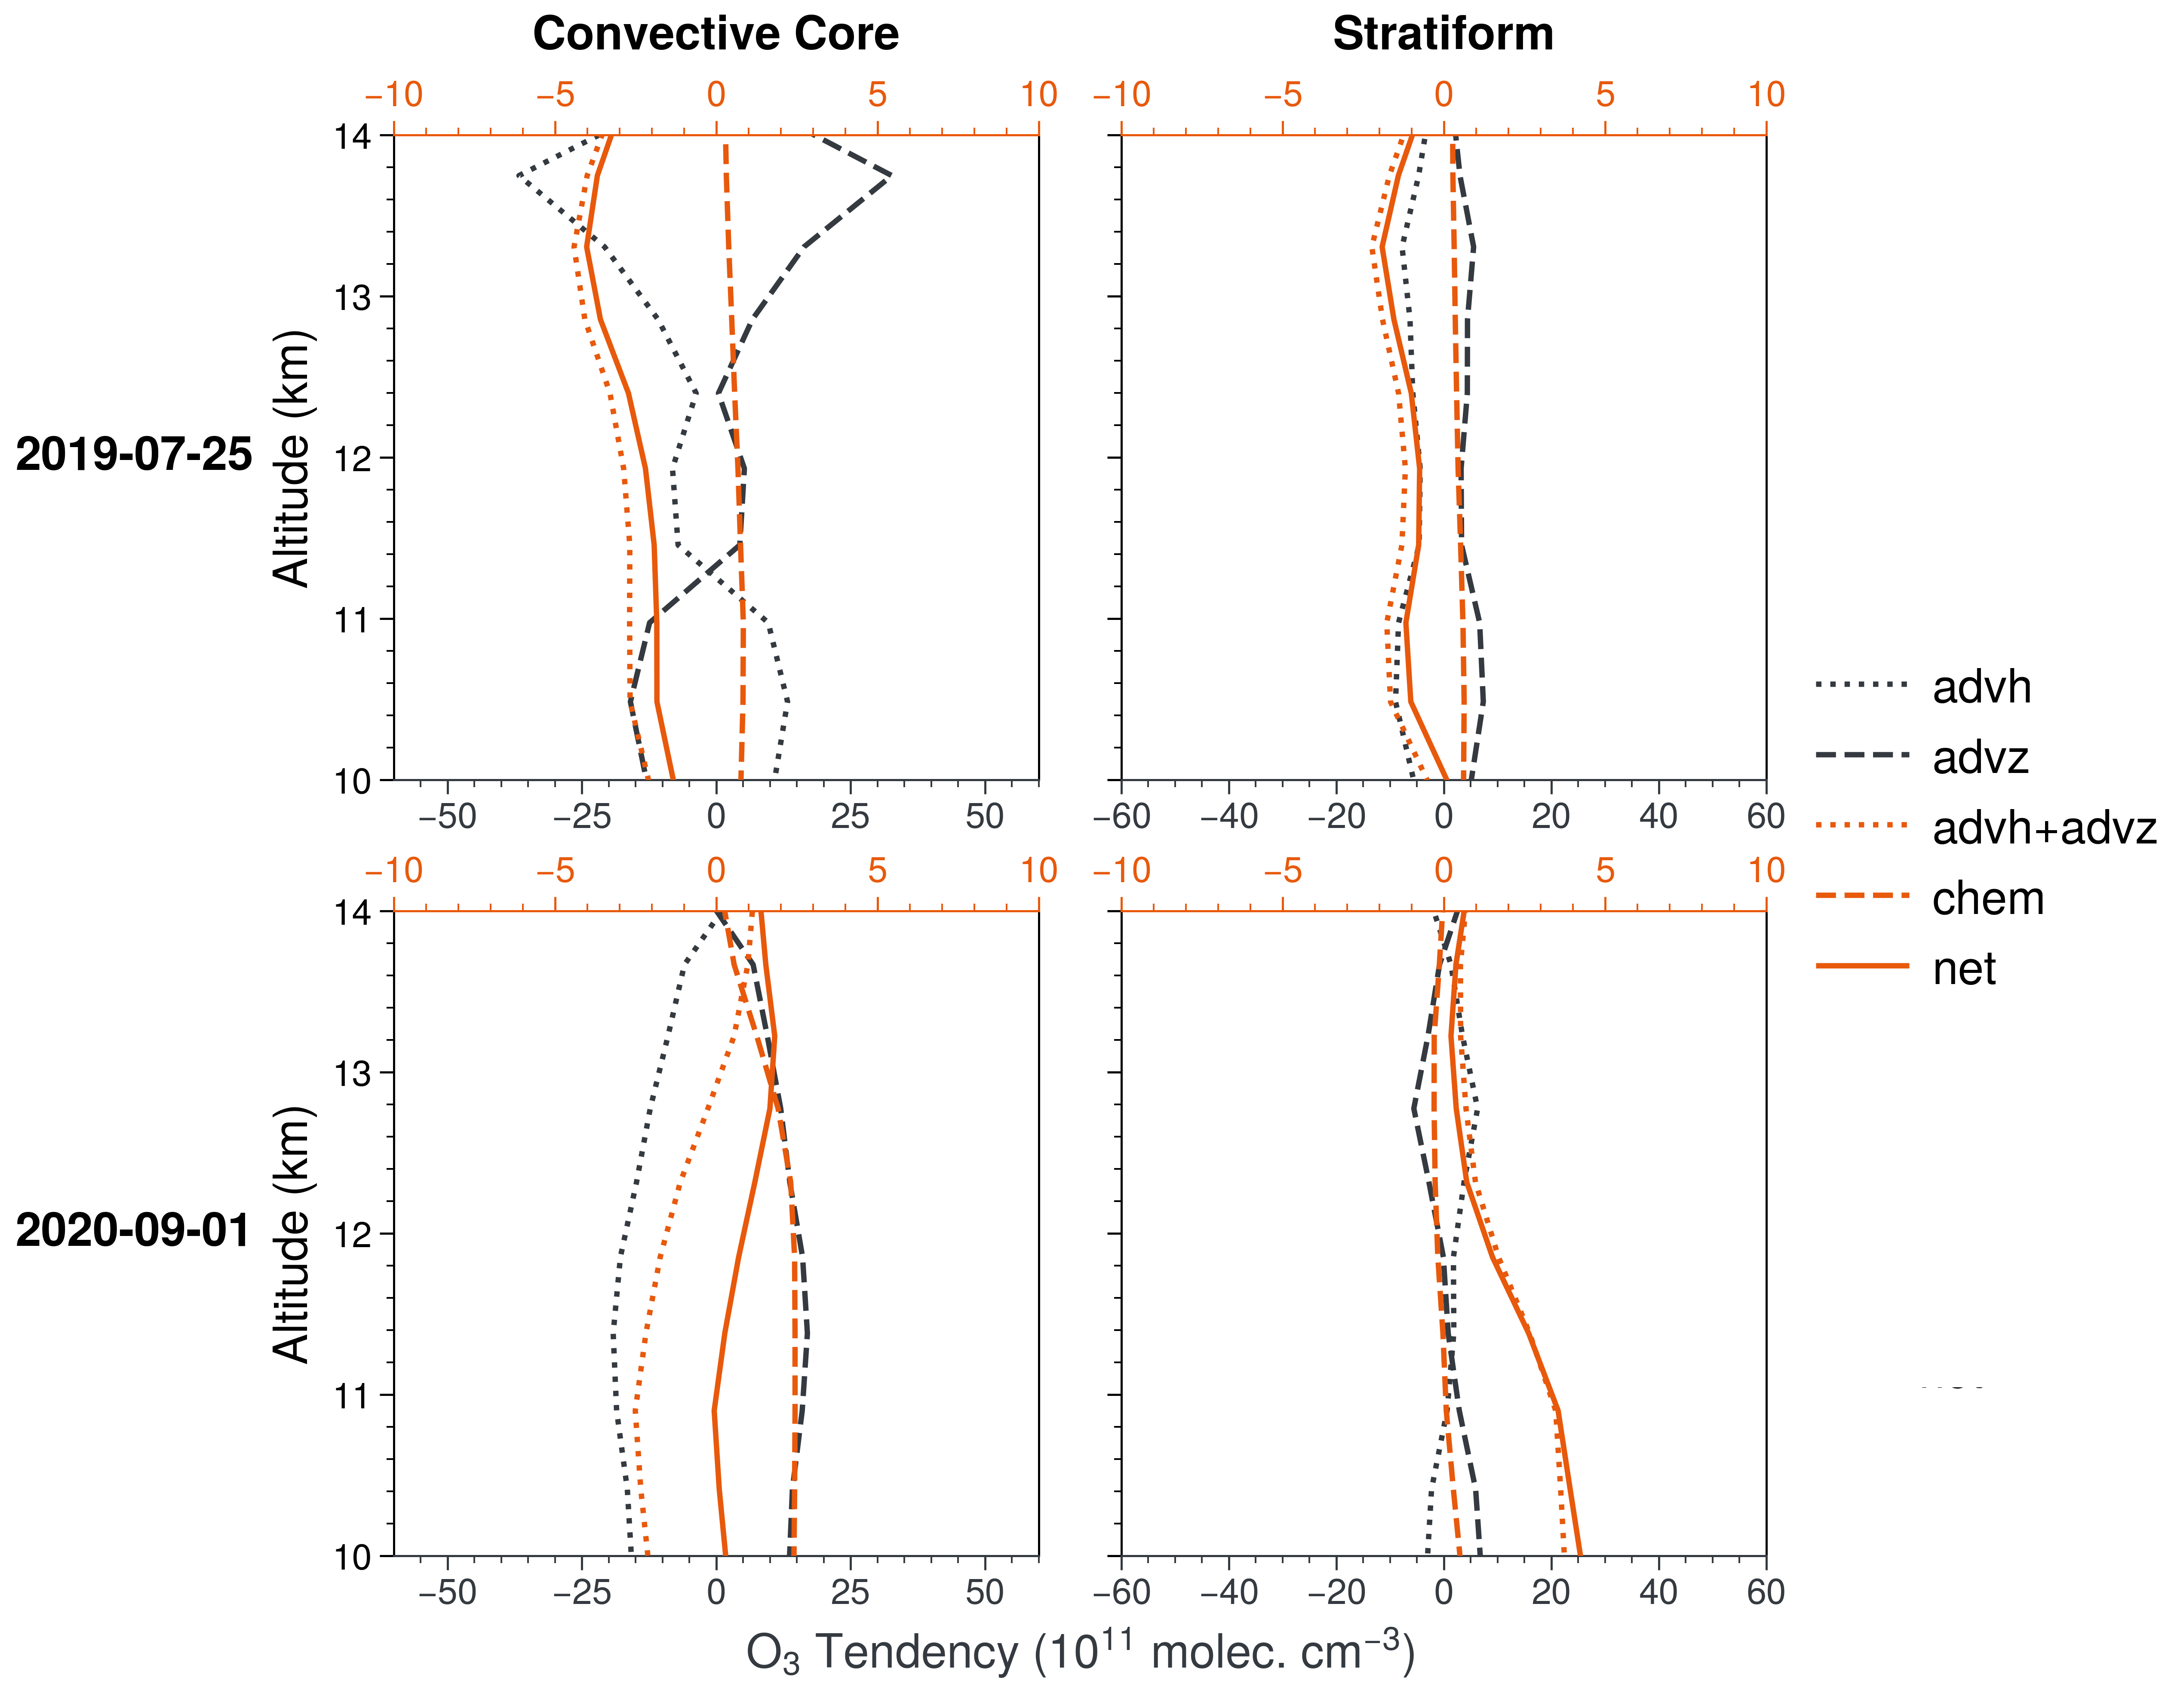
\includegraphics[width=\textwidth]{./figures/tendency_o3_classification.png}
\caption{
对流旺盛期间水平输送(advh)、垂直输送(advz)和化学贡献(chem)在对流核和层云区内导致的O$_{\ch{3}}$净产率垂直分布。
\\
Figure \ref{fig:tendency_o3_classification}. The vertical distributions of the O$_{\ch{3}}$ net production rate and tendency in the convective and stratiform regions, due to horizontal advection (advh), vertical advection (advz), and chemistry (chem) during the convective periods.
}
\label{fig:tendency_o3_classification}
\end{figure}

由以上的中国东南部O$_{\ch{3}}$浓度变化分析可知化学贡献的重要性,
因此我们进一步利用MERRA2-GMI的3小时平均模式结果,分析了动力(大尺度输送)、物理(湍流和对流)和化学对中低纬度O$_{\ch{3}}$的贡献。
如图\ref{fig:uto3_tendency}所示,中低纬度的O$_{\ch{3}}$趋势主要由动力项主导,且噪点较多,
物理的贡献主要为负,代表低O$_{\ch{3}}$浓度的空气向对流层上层输送。
然而在污染地区(如美国东南部、非洲中部、印度北部以及中国东南部)化学贡献的正贡献占主导,表明O$_{\ch{3}}$的净生成。
由于对流和闪电产生较高浓度的NO$_{\ch{2}}$,这些区域的正化学贡献在阴天比晴天高50--160\%(图\ref{fig:uto3_chem_tendency})。
该结果与中国东南部O$_{\ch{3}}$在整个对流生命期的变化及来源相符,突出了LNO$_{\ch{2}}$对于夏季对流层上层O$_{\ch{3}}$浓度的长期影响。


\begin{figure}[H]
    \centering
    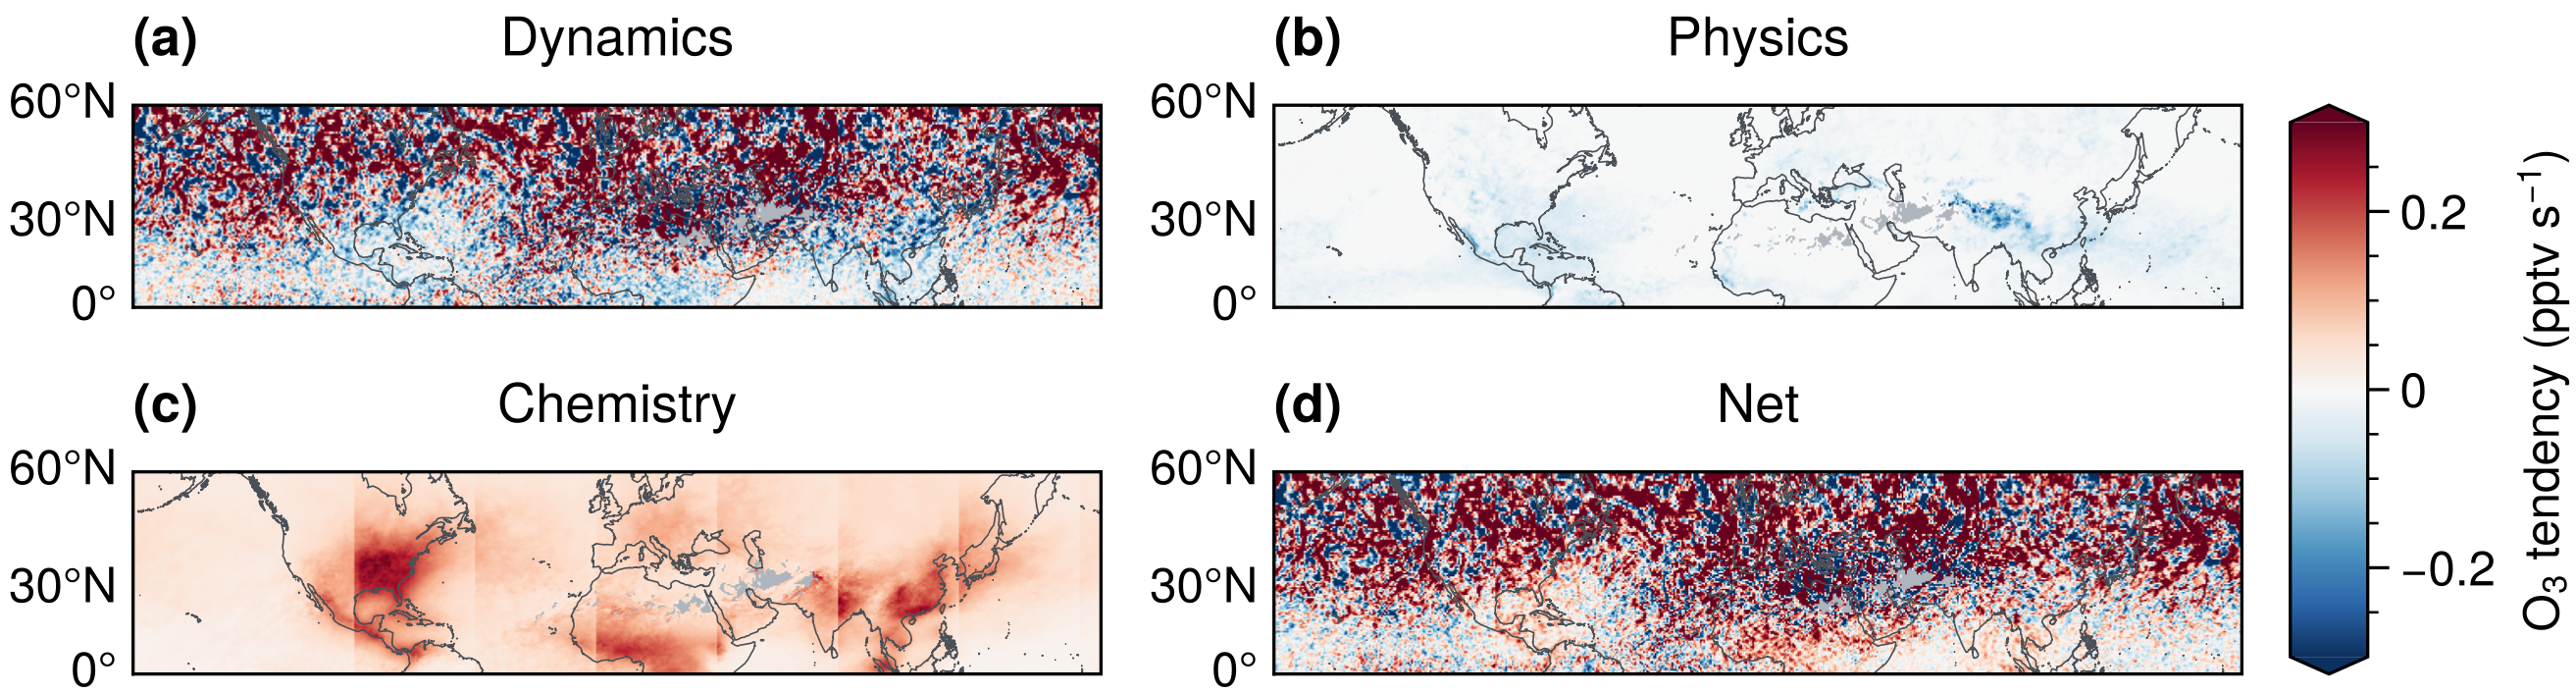
\includegraphics[width=0.8\textwidth]{./figures/uto3_tendency.png}
    \caption{
    2019年6--8月北半球中低纬度MERRA2-GMI模拟的261 hPa高度O$_{\ch{3}}$的平均趋势:
    (a)动力;(b)物理;(c)化学;(d)净趋势。\\
    Figure \ref{fig:uto3_tendency}. The mean tendency of O$_{\ch{3}}$ simulated by MERRA2-GMI at 261 hPa due to (a) dynamics, (b) physics, (c) chemistry, and (d) net tendency at the northern middle-low latitudes for June--August in 2019.
    }
    \label{fig:uto3_tendency}
\end{figure}


\begin{figure}[H]
    \centering
    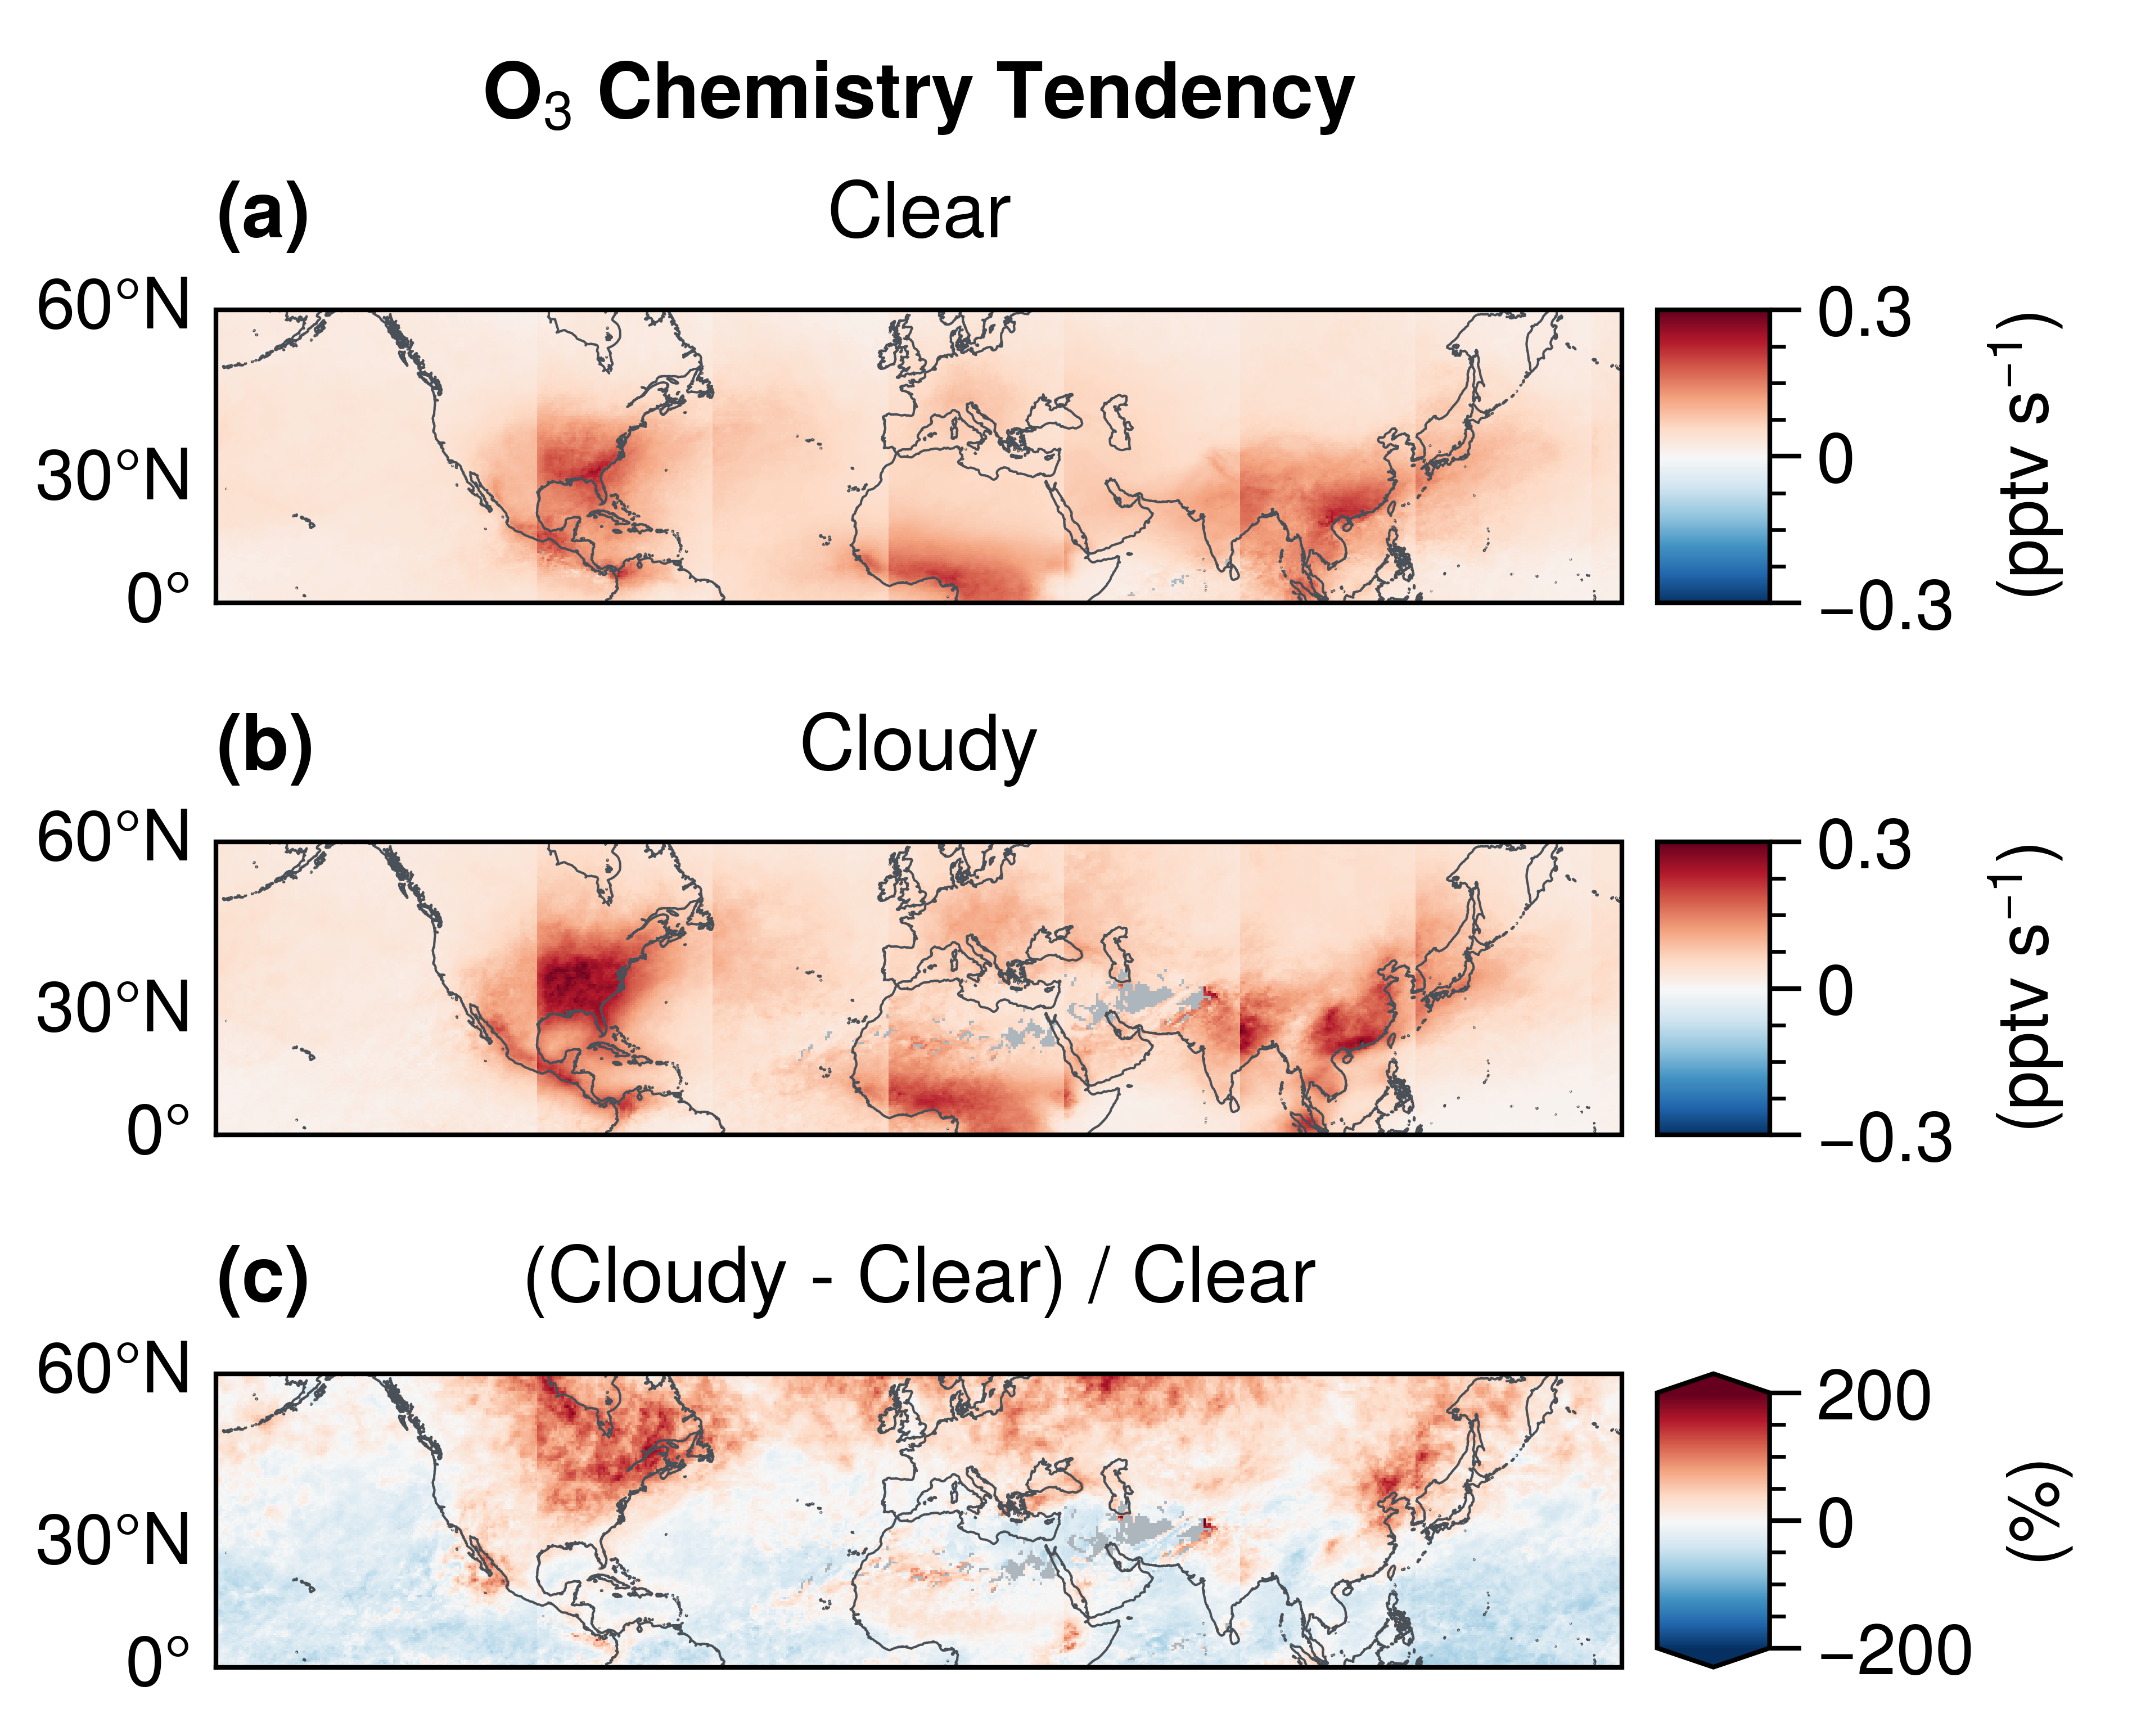
\includegraphics[width=\textwidth]{./figures/uto3_chem_tendency.png}
    \caption{
    2019年6--8月北半球中低纬度MERRA2-GMI模拟的261 hPa高度O$_{\ch{3}}$的平均化学趋势:
    (a)晴空条件;(b)有云条件;(c)两者的相对差。\\
    Figure \ref{fig:uto3_chem_tendency}. The mean chemistry tendency of O$_{\ch{3}}$ simulated by MERRA2-GMI for 261 hPa at the northern middle-low latitudes for June--August in 2019:
    (a) clear condition, (b) cloudy condition, and (c) percentage differences.
    }
    \label{fig:uto3_chem_tendency}
\end{figure}

\subsection{闪电氮氧化物的贡献} \label{sec:lnox_effects}

我们将开启和关闭LNO排放所得到的中国东南部O$_{\ch{3}}$累计物理变化速率(IPR)进行对比,
从而得到LNO$_{\ch{x}}$对O$_{\ch{3}}$的影响(表\ref{table:ipr})。
如上节所述,化学的正贡献主导了整个对流生命期间O$_{\ch{3}}$浓度的变化,是对流输送贡献的5--10倍。
在2019年个例的对流旺盛期和整个生命周期中,LNO$_{\ch{x}}$使得O$_{\ch{3}}$的净产量分别降低了25\%和40\%。
此外LNO$_{\ch{x}}$虽然促使对流核心区的O$_3$化学产量增加125\%,但净产量下降21\%(表\ref{table:ipr_classification}),而LNO$_{\ch{x}}$在层云区域对O$_3$的影响小于4\%。
而对于2020年个例,由于站点附近闪电密度较小,化学贡献导致的O$_{\ch{3}}$浓度变化不显著($\leq$1\%)。
% 而前人研究表明,LNO$_{\ch{x}}$在日尺度范围内可提高下风向的O$_{\ch{3}}$产量\citep{Pickering.1996,DeCaria.2005}。
% 因此,有必要准确估计LNO$_{\ch{x}}$的产率(见第\ref{chapter:PE}章)。


\begin{table*}[h]
\centering
\caption{探空所经区域的O$_{\ch{3}}$平均累积趋势(10--14 km)\\ Table \ref{table:ipr} Process analysis table for the mean O$_{\ch{3}}$ integrated tendencies (10--14 km)}
\footnotesize
{\centering
\renewcommand{\arraystretch}{1}
\begin{tabular}{@{\extracolsep{\fill}} cccccc}
\thickline
  阶段           & 时间             & 闪电NO排放 (mol/flash) & 输送贡献$^a$       & 化学贡献$^a$              & 净变化$^a$    \\
\thickline
整个生命期         & 2019-07-25       & 0               & -3.3 (-24.6 \%)        & 16.7 (124.6 \%)        & 13.4       \\
                   & (03:20--05:40)   & 500             & -2.3 (-28.8 \%)        & 10.3 (128.8 \%)        & 8.0        \\
\cline{2-6}
                   & 2020-09-01       & 0               & 3.4  (9.6 \%)          & 32.0 (90.4 \%)         & 35.4       \\
                   & (04:20--06:40)   & 500             & 4.4  (12.1 \%)         & 31.9 (87.8 \%)         & 36.3       \\
\hline
对流旺盛期   & 2019-07-25      & 0              & -19.6 (140.0 \%)       & 5.6 (-40.0 \%)         & -14.0      \\
                    & (04:20--05:00)  & 500            & -20.0 (114.3 \%)       & 2.5 (-14.3 \% )        & -17.5      \\
\cline{2-6}
                    & 2020-09-01      & 0              & -9.7  (-131.1 \%)      & 17.1 (231.1 \% )       & 7.4        \\
                    & (05:40--06:20)  & 500            & -10.1 (-148.5 \%)      & 16.9 (248.5 \% )       & 6.8        \\
\thickline
\end{tabular}
\par }
\begin{tablenotes}
\linespread{1}\footnotesize
\item $^{a}$ 单位是 10$^{10}$ molec. cm$^{-3}$。百分比是每种贡献在净O$_{\ch{3}}$变化中的比例。 \\
\item $^{a}$ The unit is 10$^{10}$ molec. cm$^{-3}$. The percentage is the proportion of each part in the net O$_{\ch{3}}$ change.
\end{tablenotes}
\label{table:ipr}
\end{table*}




\begin{table*}[h]
\centering
\caption{对流旺盛期间对流核心区和层云区的O$_{\ch{3}}$平均累积趋势过程分析(10--14 km)\\ Table \ref{table:ipr} Process analysis table for the mean O$_{\ch{3}}$ integrated tendencies (10--14 km) at convective and stratiform regions during the convective periods}
\footnotesize
{\centering
\renewcommand{\arraystretch}{1}
\begin{tabular}{@{\extracolsep{\fill}} cccccc}
\thickline
  区域           & Time                & 闪电NO排放 (mol/flash) & 输送贡献$^a$       & 化学贡献$^a$              & 净变化$^a$    \\
\thickline
对流核心区         & 2019-07-25         & 0               & -23.9 (113.3 \%)        & 2.8 (-13.3 \%)        & -21.1       \\
                   & (04:20--05:00)   & 500             & -31.9 (124.6 \%)        & 6.3 (-24.6 \%)        & -25.6        \\
\cline{2-6}
                   & 2020-09-01       & 0               & -11.3  (-127.0 \%)          & 20.2 (227.0 \%)         & 8.9       \\
                   & (05:40--06:20)   & 500             & -10.7  (-117.6 \%)         & 19.8 (217.6 \%)         & 9.1       \\
\hline
层云区               & 2019-07-25      & 0              & -14 (150.5 \%)       & 4.7 (-50.5 \%)         & -9.3      \\
                    & (04:20--05:00)  & 500            & -15.2 (143.4 \%)       & 4.6 (-43.4 \% )        & -10.6      \\
\cline{2-6}
                    & 2020-09-01      & 0              & 17.2  (107.5 \%)      & -1.2 (-7.5 \% )       & 16.0        \\
                    & (05:40--06:20)  & 500            & 17.7 (106.6 \%)      & -1.1 (-6.6 \% )       & 16.6        \\
\thickline
\end{tabular}
\par }
\begin{tablenotes}
\linespread{1}\footnotesize
\item $^{a}$ 单位是 10$^{10}$ molec. cm$^{-3}$。百分比是每种贡献在净O$_{\ch{3}}$变化中的比例。 \\
\item $^{a}$ The unit is 10$^{10}$ molec. cm$^{-3}$. The percentage is the proportion of each part in the net O$_{\ch{3}}$ change.
\end{tablenotes}
\label{table:ipr_classification}
\end{table*}

% 此外,我们利用TROPOMI数据将对流分为三个区域:新生闪电区、闪电下风向和闪电老化区(详见\ref{sec:lnox_affects_tropomi}节和图\ref{fig:china_s5p_amf_diff})。
% 首先基于不同LNO产率的模拟结果,获得O$_{\ch{3}}$差异($\Delta$O$_{\ch{3}}$)的廓线(图\ref{fig:irr_timeseries}a--c)。
% $\Delta$O$_{\ch{3}}$在2--5 km之间大部分为正($<$1 ppbv),在5--12 km 之间为负($>$-3 ppbv),
% 这与\citet{Ott.2007}研究中所有高度上O$_{\ch{3}}$都产生净损失($>$-4 ppbv)的结论不一致。
% 此外,较高的LNO产率(700 mol 每闪电)与默认500 mol 每闪电的结果相比,所有高度的O$_{\ch{3}}$浓度均降低,
% 甚至导致闪电下风向2--5 km高度的$\Delta$O$_{\ch{3}}$由正转负(图\ref{fig:irr_timeseries}b)。
% 由于LNO$_{\ch{x}}$在8--10 km高度达到峰值,O$_{\ch{3}}$浓度也在此层降低最多。%(2.6 ppbv)。

% \setlength{\abovedisplayskip}{3pt} % decrease space before equation
% \setlength{\belowdisplayskip}{3pt} % decrease space after equation
接着,我们以受LNO$_{\ch{2}}$影响更大的2019年为例,利用积分反应速率(IRR)来评估LNO$_{\ch{x}}$对$\Delta$O$_{\ch{3}}$的影响,以及O$_{\ch{3}}$变化的化学机制。
% 我们分两层来看该影响,因为800--500 hPa上$\Delta$O$_{\ch{3}}$为正,500--200 hPa上$\Delta$O$_{\ch{3}}$为负。
对流层O$_{\ch{3}}$主要由以下反应速率项控制\citep{Mazzuca.2016}:
{
\abovedisplayskip=3pt%
\belowdisplayskip=3pt%
\begingroup
\allowdisplaybreaks
\begin{align}
  \frac{d}{dt}[\mathrm{O_3}] &= k_1[\mathrm{NO}][\mathrm{HO_2}] + \sum_{i}  k_i[\mathrm{NO}][\mathrm{R_iO_2}] - k_3[\mathrm{OH}][\mathrm{NO_2}][\mathrm{M}] - P(\mathrm{RONO_2}) \nonumber \\
                             & - k_4[\mathrm{HO_2}][\mathrm{O_3}] - k_5[\mathrm{OH}][\mathrm{O_3}] - k_6[\mathrm{H_2O}][\mathrm{O(^1D)}] - L(\mathrm{O_3+alkenes})
\end{align}
\endgroup
}

其中k$_i$是过氧自由基(R$_i$O$_{\ch{2}}$)与NO之间的反应速率系数,
$P(\ch{RONO2})$为硝酸盐生成反应,
$L(\mathrm{O_3+alkenes})$为烯烃消耗O$_{\ch{3}}$的反应。
由于OH+NO$_{\ch{2}}$、O$_{\ch{3}}$+HO$_{\ch{2}}$和O(1D)+H$_2$O共占O$_{\ch{3}}$化学消耗的85--95\%,
故IRR时间序列图(图\ref{fig:irr_timeseries})除O$_{\ch{3}}$生成反应外,仅包含了此三种消耗反应。
由于2019年对流个例的垂直运动剧烈(见\ref{sec:convec_impacts}节),
故净积分反应速率的时间序列变化可达1.8$\times$10$^7$ molec. cm$^{-3}$ s$^{-1}$,且O$_{\ch{3}}$净化学产量保持正值。
总体而言,整个生命期间LNO$_{\ch{2}}$的排放导致对流层上层O$_{\ch{3}}$化学总生成量降低4\%,
总损耗量增加23\%。
具体而言,NO+HO$_{\ch{2}}$之间的正贡献始终占主导地位(75--80\%),
而另一正贡献即RO$_{\ch{2}}$对NO的氧化占20--25\%,该两种反应的IRR在LNO的作用下,均在对流旺盛期增大$\sim$10\%而后降低$\sim$35\%。
对于O$_{\ch{3}}$的消耗反应而言,对流旺盛期前是O$_{\ch{3}}$+OH和OH+NO$_{\ch{2}}$占主导,且两者速率相当(1--2$\times$10$^6$ molec. cm$^{-3}$ s$^{-1}$),
而由于对流系统中LNO的排放,使得OH 和 HO$_{\ch{2}}$ 之间的平衡向OH方向移动,其中OH+NO$_{\ch{2}}$的IRR是O$_{\ch{3}}$和OH的1.2--2.8倍。


\begin{figure}[H]
\centering
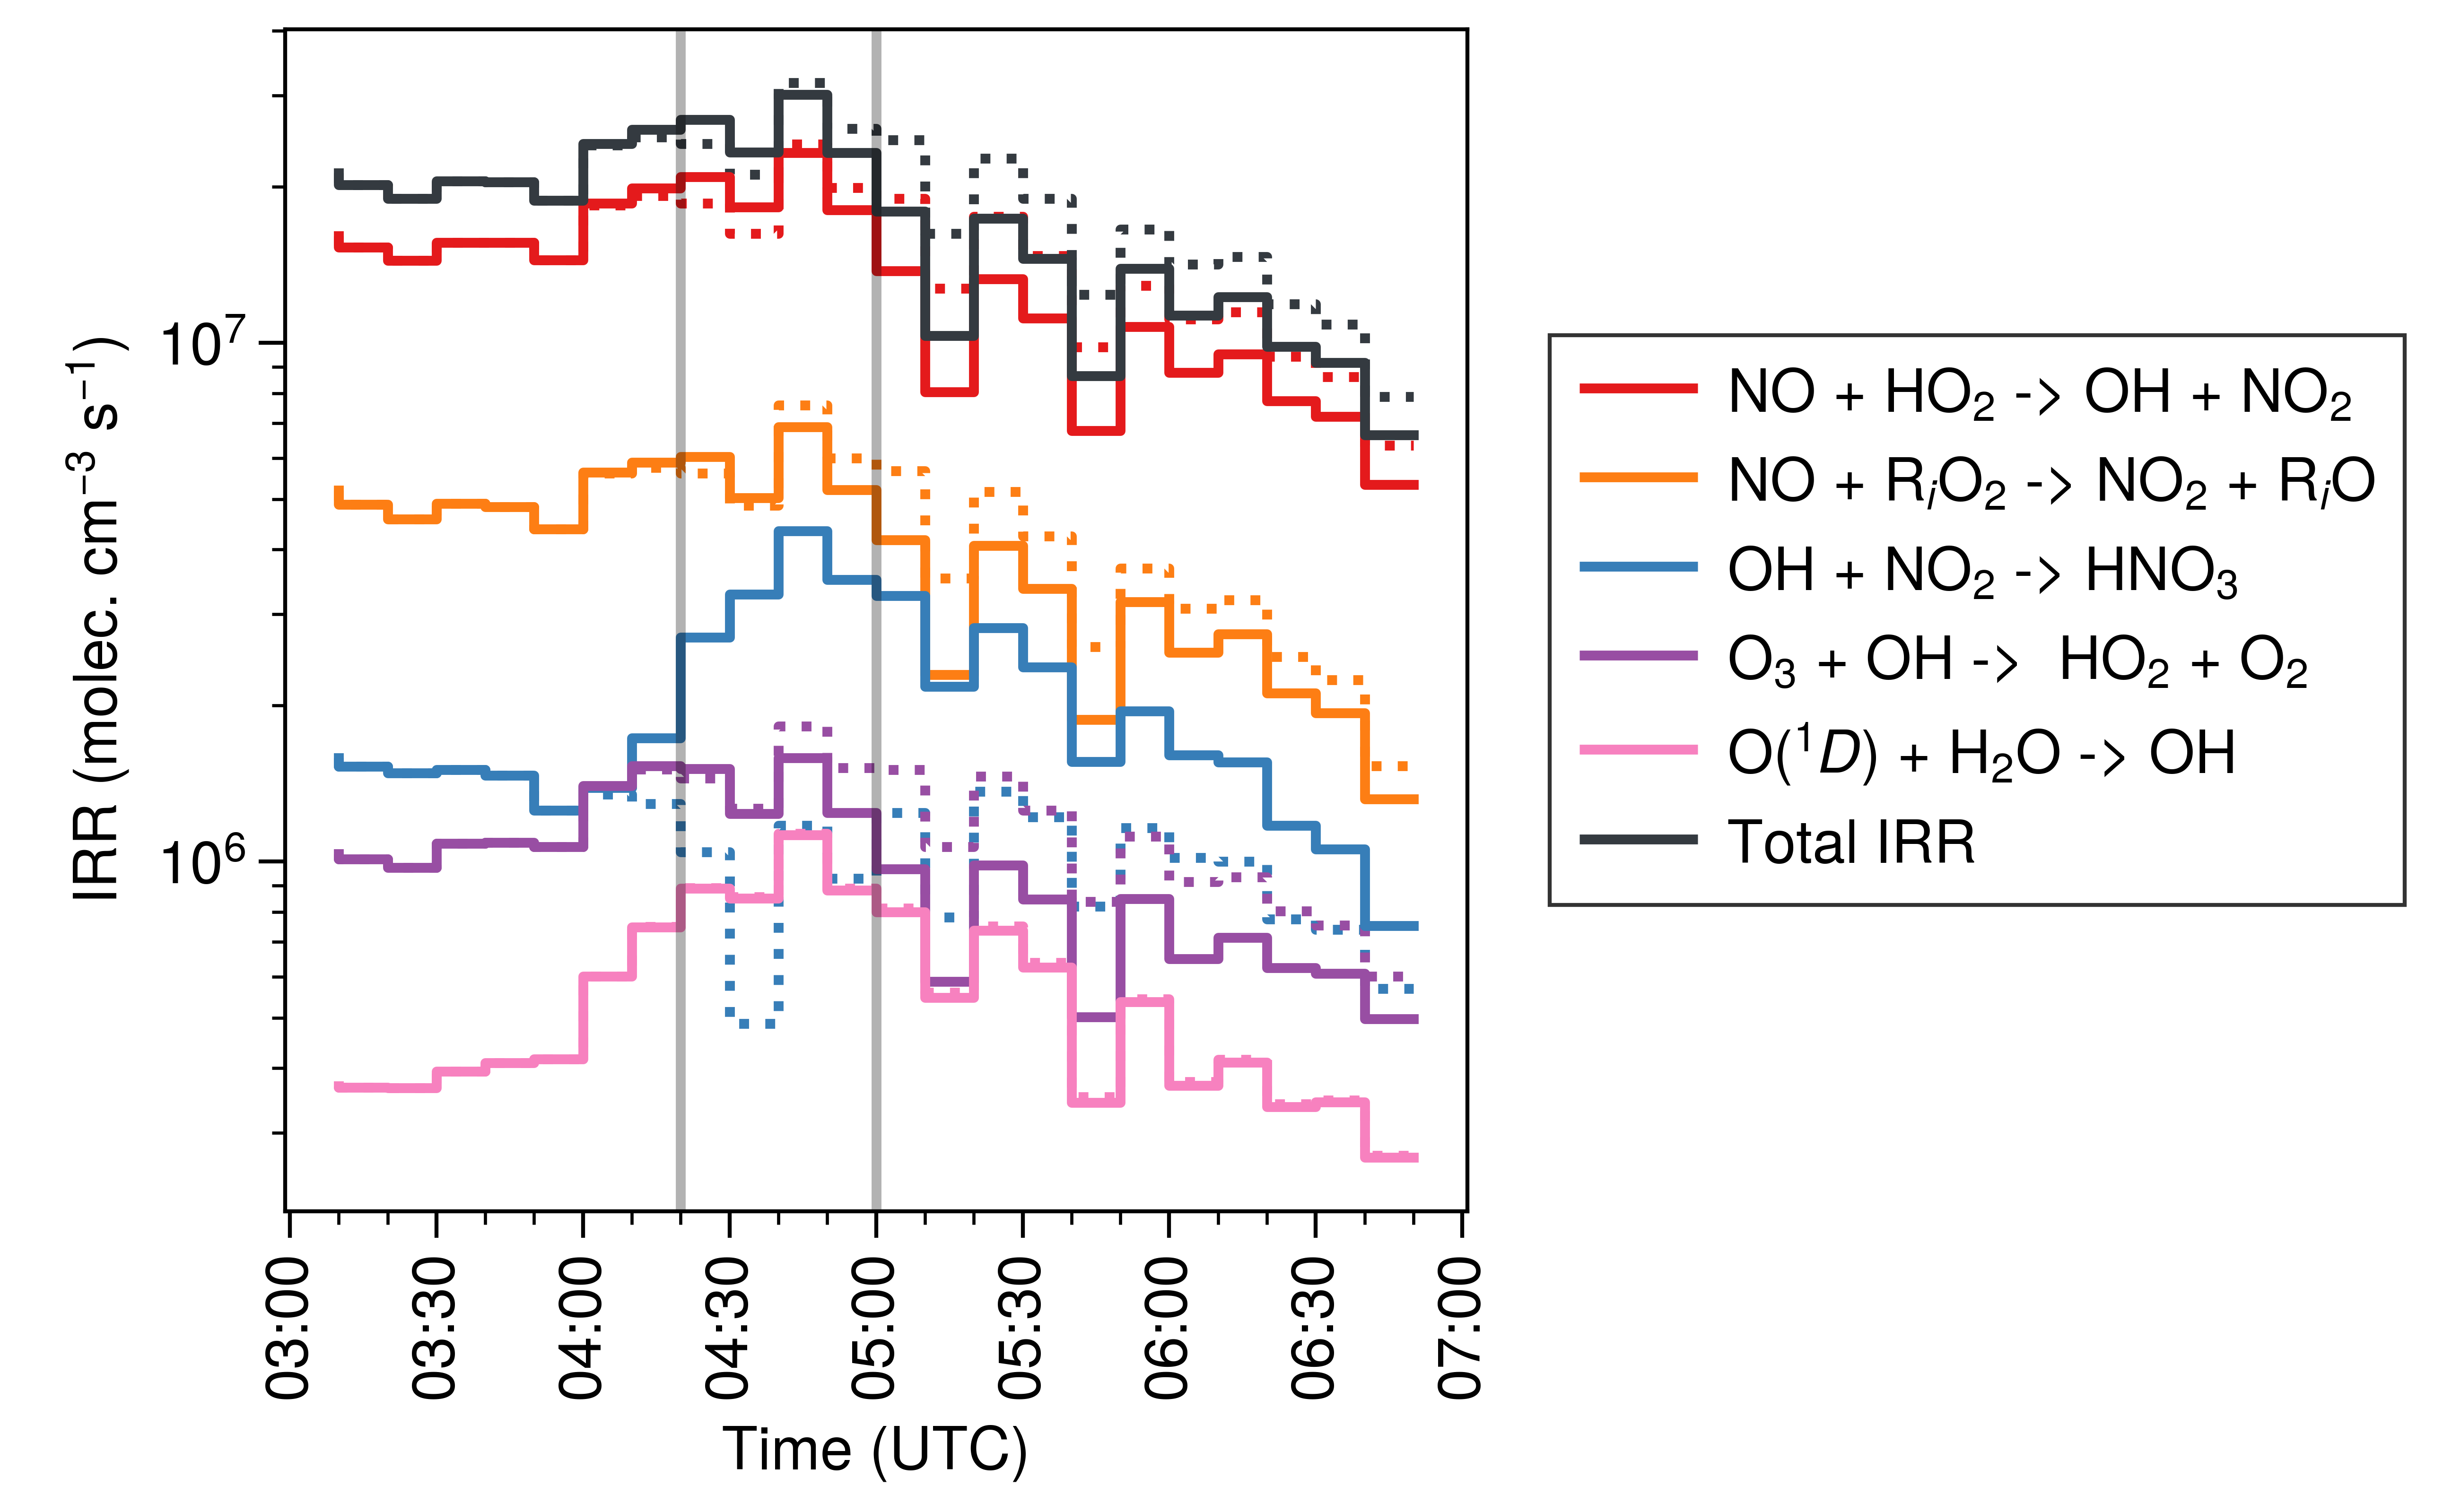
\includegraphics[width=\textwidth]{./figures/irr_timeseries.png}
\caption{
与O$_{\ch{3}}$有关的主要平均累积反应速率(IRR)在2019年个例中不同区域10--14 km高度的时间序列:
(a)臭氧探空仪所经区域,(b)对流核,(c)层云区域。
其中图例显示了详细的物种和反应,总IRR是从生成O$_{\ch{3}}$的IRR(红线和橙线)中减去O$_{\ch{3}}$损失的IRR。
实线为模拟中开启LNO(500 mol 每闪电)排放的IRR,而虚线表示关闭LNO排放。\\
Figure \ref{fig:irr_timeseries}. Time series of the mean integrated reaction rate (IRR) of reactions related to O$_{\ch{3}}$ between 10 and 14 km in different regions of 2019 case: (a) the region passed by ozonesondes, (b) convective cores, and (c) stratiform regions.
The legend shows detailed species and reactions.
The total IRR is the O$_{\ch{3}}$ loss IRR subtracted from the O$_{\ch{3}}$ production IRR (red and orange lines).
The solid line shows the IRR with LNO (500 mol/flash) while the dashed line is without LNO.
}
\label{fig:irr_timeseries}
\end{figure}
